% !TeX spellcheck = fr_FR
\chapter{Chapitre 4 : Résultats}

Ce chapitre porte sur les différents essais qui ont été effectués et les résultats de ceux-ci.
Le projet ayant été adapté en cours de route, les sous-chapitres sont organisés de manière chronologique.

\section{Adaptation du simulateur Pe Extractor}
La première étape du projet a été de maîtriser et formatter les données du premier simulateur "pe\_extractor".
Comme évoqué lors du chapitre précédent, les bacs contenant les photons détectés sont générés à une fréquence plus élevée que celle du signal.
J'ai donc commencé par regrouper les différents bacs générés sur la même période que le signal :

\begin{lstlisting}[language=iPython,caption={Regroupement des bacs de photons-électrons, signal\_sense.ipynb},captionpos=b]
# generator variables
n_sample = 200000
n_sample_init = 0
batch_size = 1
shift_proba_bin = 30
sigma_smooth_pe_ns = 0
bin_size_ns = 0.20
sampling_rate_mhz = 1000 #200 MHz is the sampling rate of Terzina
				#1000 LST + MST
pe_rate_mhz = 150 # 1 to 150 MHz
noise_lsb=4. # 3.5 to 5.5
amplitude_gain=16.
relative_gain_std=0.05

# computed variables
sampling_period_s = 1 / (sampling_rate_mhz * 1e6)
bin_per_sample = ceil(((sampling_period_s) * 1e9) / bin_size_ns)

# parameters omitted for brevity
gen = generator_nsb(...)
data = next(gen)

# data contains in index 0 the configurable batches of the discrete signal
# and in index 1 the batches of truth
# here we configured only 1 batch, which explains the [1][0]
summed_bins = np.sum(data[1][0].reshape(-1, bin_per_sample), axis=1)
\end{lstlisting}

\newpage
Ce qui nous donne le couple de données suivant :
\begin{figure}[tbph!]
	\centering
	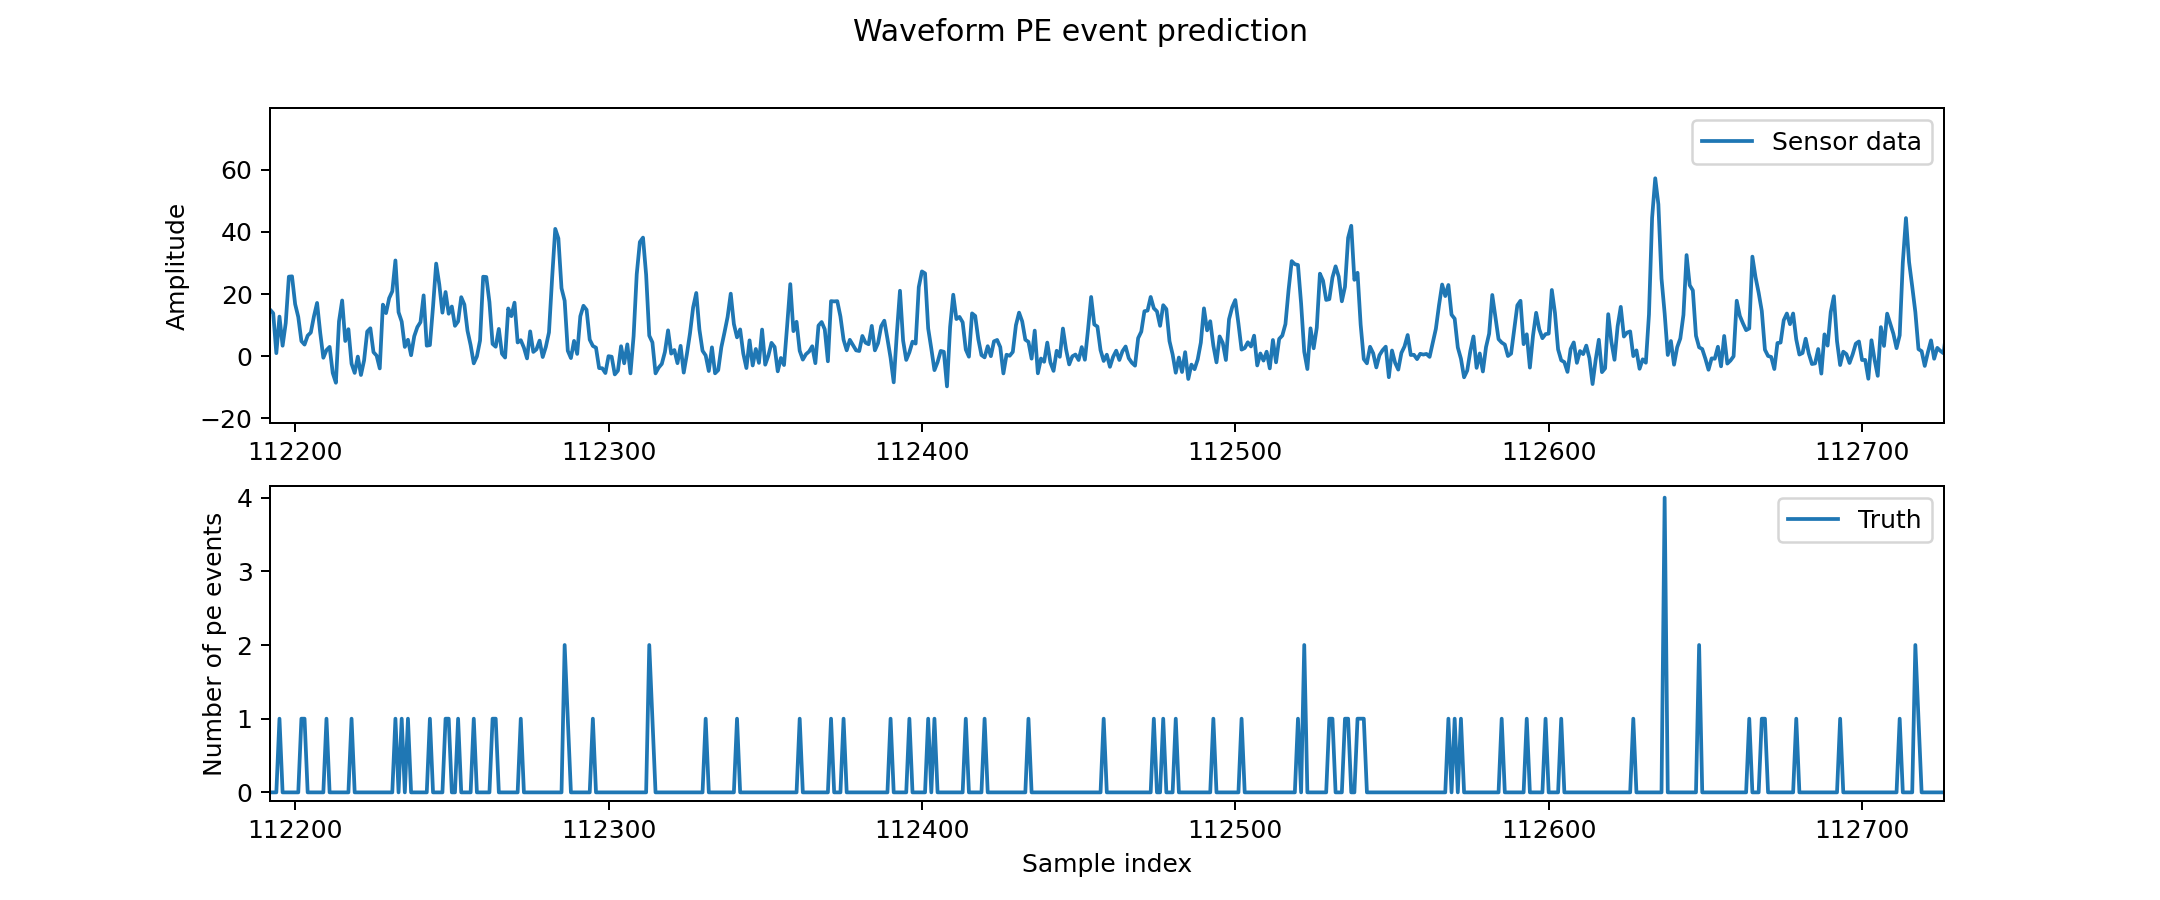
\includegraphics[width=\linewidth]{PeExtractorDataAndTruth.png}
	\caption[Exemple de données générées par "pe\_extractor"]{Exemple de données générées par "pe\_extractor".}
\end{figure}

Les configurations des paramètres du générateur sont restées majoritairement les mêmes au cours du projet;
seuls ceux commentés ont évolués au cours du projet en fonction du télescope visé. Il en va de même pour le fichier
d'impulsion correspondant au télescope.

\newpage
\subsection{Création d'un dataset}
Jusqu'à présent, les données produites sont deux signaux de $200'000$ échantillons. L'un contient l'amplitude électrique du capteur
et l'autre le compte de \gls{pe} pendant la période d'échantillonnage. Cependant, il ne serait pas facile d'entraîner un réseau
sur ce genre de données car il devrait avoir $200'000$ neurones d'entrée. Il est nécessaire de découper ces données
générées en plusieurs morceaux pour que le modèle puisse s'entraîner sur chaque cas individuellement.
Pour cela, on peut utiliser une technique connue appelée "sliding window" ou fenêtre coulissante en français.
Cela va diviser notre signal de $200'000$ échantillons en plusieurs parties, comme si l'on regardait ces données 
à travers une fenêtre que l'on déplace d'un bout à l'autre :

\begin{figure}[tbph!]
	\centering
	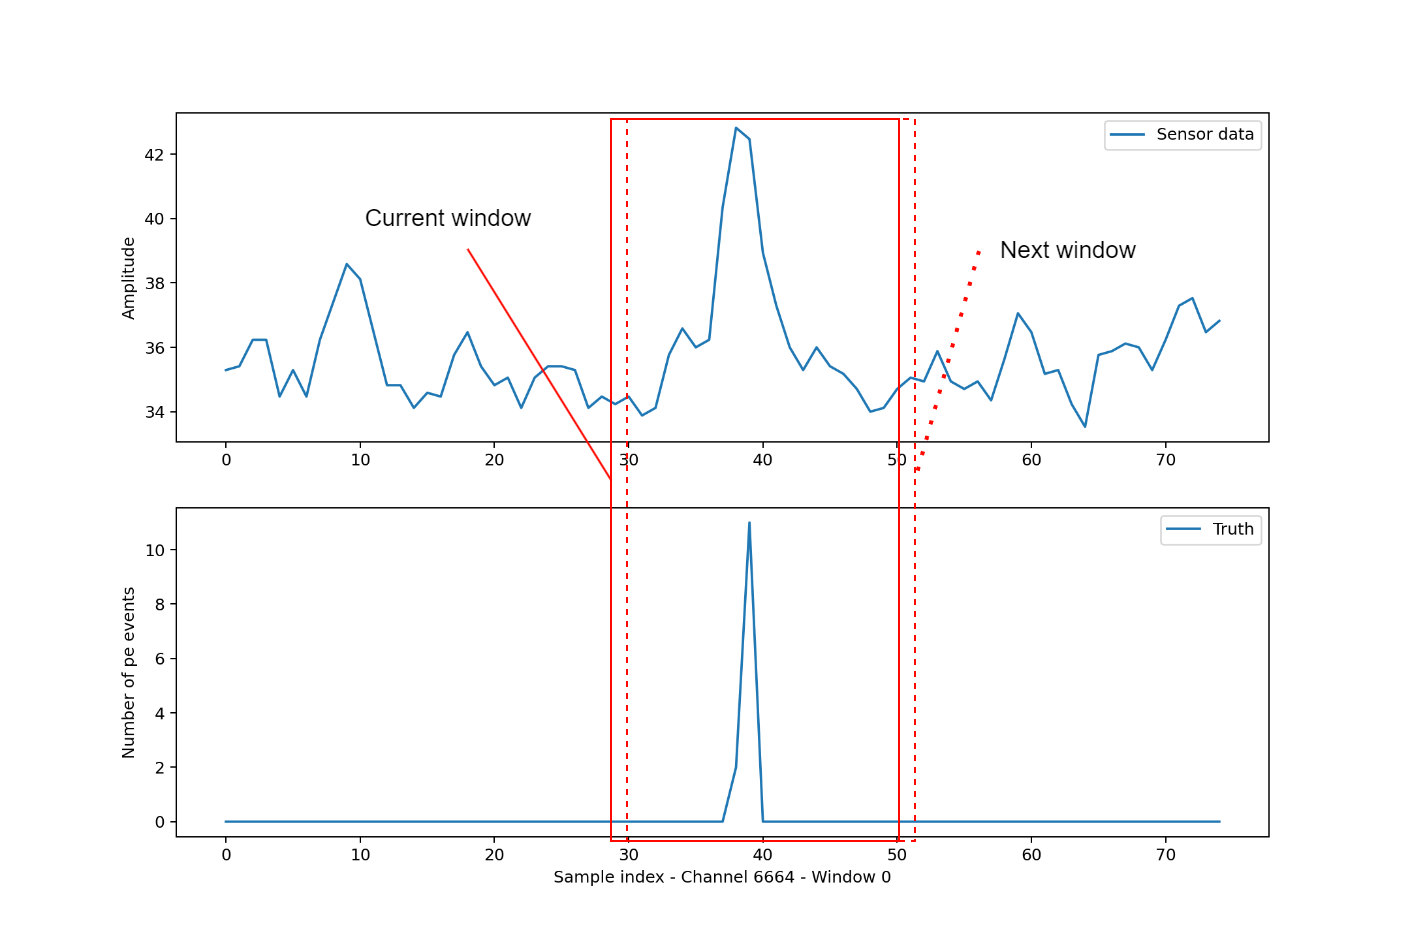
\includegraphics[width=\linewidth]{Sliding window.drawio.png}
	\caption[Exemple de séparation des données par fenêtre coulissante]{Exemple de séparation des données par fenêtre coulissante.}
\end{figure}

Cette transformation étant déjà implémentée dans la librairie Numpy, je l'ai utilisée sur les deux signaux 
en même temps afin de ne pas perdre la vérité générée par le simulateur.

À cet instant du projet, la plus grosse contrainte du réseau de neurones est qu'il doit 
fonctionner en temps réel, avec le moins d'utilisation de ressources, à bord de Terzina.
C'est pour cela qu'au début des tests, plusieurs tailles de fenêtres ont été testées, 7, 11, 21 
jusqu'à un maximum de 51; au delà, cela était jugé excessif.
De plus, la conception des \gls{asic} prévoyait de ne numériser qu'environ une vingtaine d'échantillons lors d'un déclenchement.

\section{Premiers tests de réseaux neuronaux}

\subsection{Détection booléenne de photon-électron}
Comme premier réseau neuronal, j'ai essayé de détecter la présence 
ou non d'au moins un \gls{pe} exactement au centre de chaque fenêtre.

Le résultat attendu de ce réseau est une seule estimation en sortie de la présence ou non d'un photon à l'échantillon central.
Pour cela, les fenêtres de vérité ont été converties en un tableau de taille 1 avec la valeur 1 ou 0 dépendant de la présence d'au moins un \gls{pe}.
J'ai ensuite entraîné le réseau neuronal suivant sur ces données : 
\begin{figure}[tbph!]
	\centering
	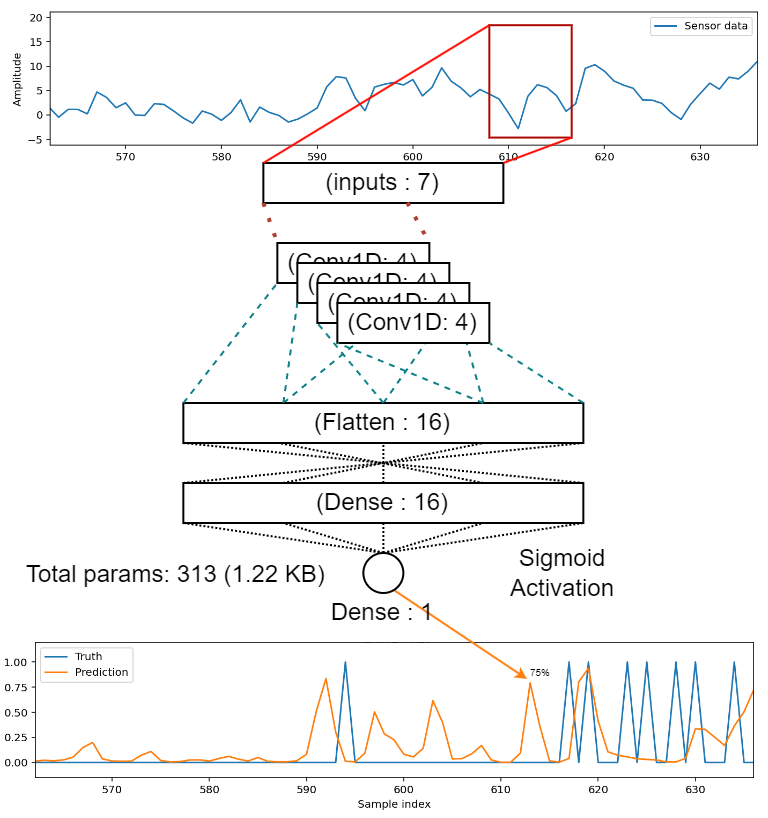
\includegraphics[width=0.6\linewidth]{cnn_simple.drawio.png}
	\caption[Diagramme d'architecture du premier CNN à classification simple]{Diagramme d'architecture du premier CNN à classification simple.}
\end{figure}

Les résultats observés provenant de cette architecture n'étaient pas bons.
La raison principale de ces mauvais résultats est l'un des pièges les plus commun du machine learning : de mauvaises données.
Cette première erreur provenait de la transformation supplémentaire pour créer des valeurs attendues booléennes.
Lors de cette transformation, une simple erreur d'indice avait récupéré le premier échantillon de la fenêtre au lieu de l'échantillon central.
Cela a donc faussé toutes les données sur lesquelles le réseau s'était entraîné.

Cette première expérience m'a poussé à développer des vues au "cas par cas" où chaque inférence du modèle peut être examinée en détail.
Cette vue affiche les données d'entrée, la vérité attendue et le résultat du modèle, ce qui permet de visualiser son comportement après entraînement. 

\begin{figure}[tbph!]
	\centering
	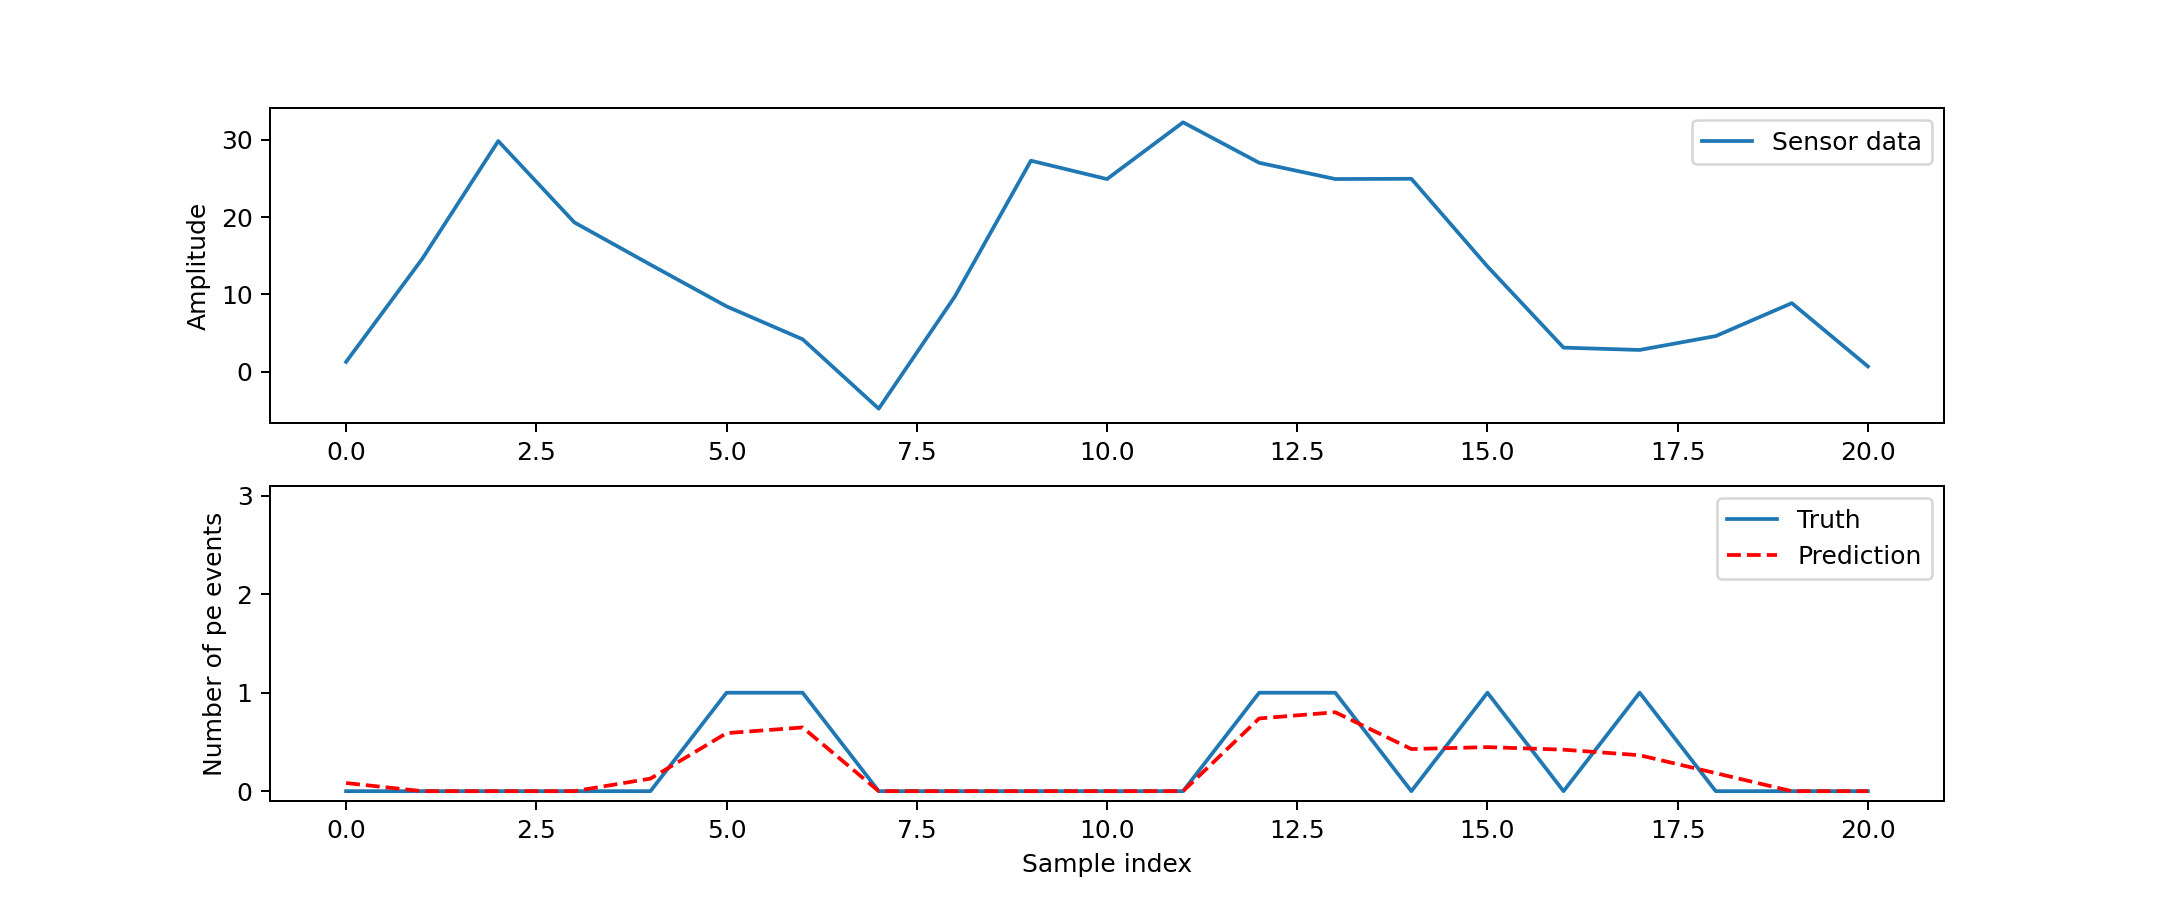
\includegraphics[width=\linewidth]{CNNWindowVisualisation.png}
	\caption[Exemple de visualisation d'une inférence d'un réseau]{Exemple de visualisation d'une inférence d'un réseau.}
\end{figure}

Cependant, même après avoir corrigé le dataset d'entraînement, les résultats -bien que légèrement améliorés- restaient non fiables à cause de nombreux
faux positifs et faux négatifs.

\subsection{Estimation calorimétrique de photon-électron par régression}
Pour avoir un meilleur point de décision qu'une simple valeur booléenne à bord de Terzina et pour améliorer les performances du premier réseau,
j'ai adapté celui-ci pour avoir une fenêtre de sortie estimant une quantité de photons présents à chaque échantillon.

En premier, il faut modifier la couche de sortie pour qu'elle ait le même nombre de neurones que la couche d'entrée. 
En plus de cela, il faut changer la fonction d'activation utilisée par les neurones de sortie.
Par défaut, la fonction utilisée est la sigmoïde. Celle-ci ne retourne que des valeurs dans l'intervalle $ \left[ 0, 1\right] $,
tandis que la fonction "ReLU" retourne des valeurs dans l'intervalle $ \left[0, +\infty\right[ $, ce qui est parafait pour compter
des \gls{pe}.

Pour l'entraînement de ce réseau, il a été choisi d'utiliser la fonction d'erreur "MeanSquaredError" et l'optimiseur Adam, car ce
sont ceux qui, après quelques tests manuels, présentaient les meilleures performances d'entraînement. 
Le dataset d'entraînement comportait  $160'000$ fenêtres et $40'000$ réservées à la validation (un répartition 80/20),
ces fenêtres étaient générées de manière aléatoire mais avec les mêmes configurations.

Ce nouveau modèle est donc capable d'estimer le nombre de \gls{pe} pour chaque échantillon.
Celui-ci a immédiatement mieux performé que le précédent :

\begin{figure}[tbph!]
	\centering
	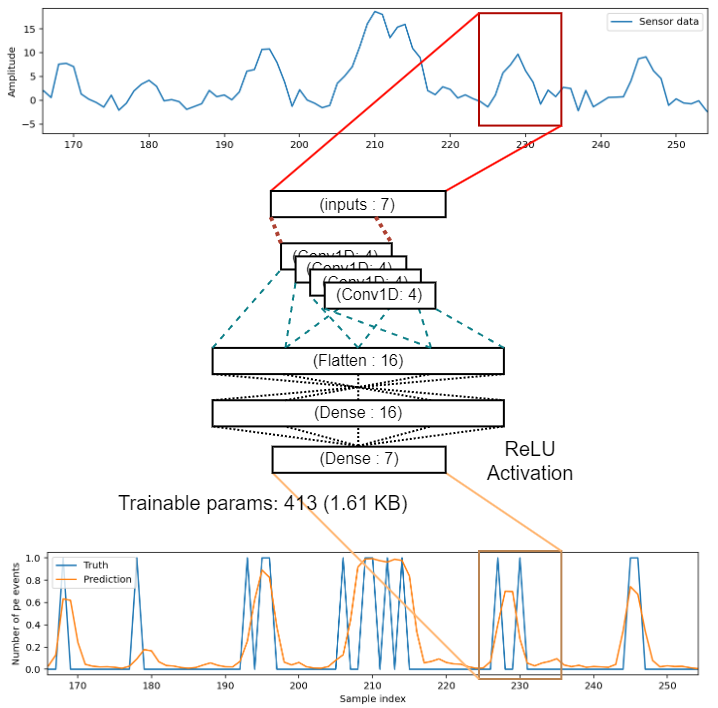
\includegraphics[width=0.8\linewidth]{cnn_mult.drawio.png}
	\caption[Diagramme d'architecture du CNN à multiples sorties]{Diagramme d'architecture du CNN à multiples sorties.}
\end{figure}

\subsection{Métriques de performance des réseaux}
Arrivé à cette étape, il est devenu nécessaire de quantifier les écarts de performances entre chaque architecture testée.
Pour des modèles effectuant de la classification, chaque prédiction peut être comptabilisée dans une matrice de confusion comme celle-ci :
\newpage
\begin{figure}[tbph!]
	\centering
	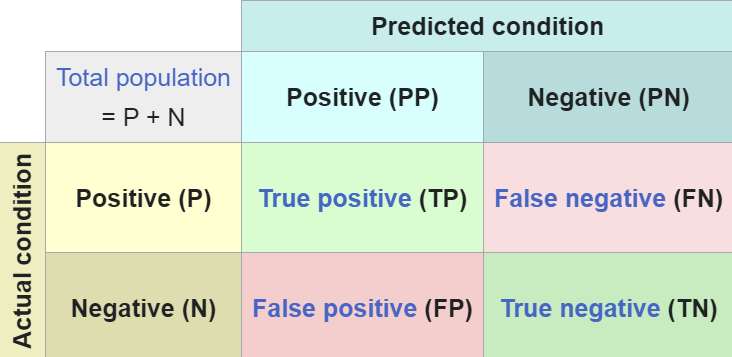
\includegraphics[width=0.6\linewidth]{ConfusionMatrix.png}
	\caption[Matrice de confusion]{Matrice de confusion. Source : \cite{ConfusionMatrixImage}}
\end{figure}

Dans notre cas, nous n'effectuons pas une classification mais une régression.
Pour pouvoir remplir une matrice de confusion, il est nécessaire de définir ce qu'est un vrai positif, un faux positif, etc.
J'ai donc défini que, si l'estimation du modèle dépasse une valeur de 0.5, cette estimation
est considérée comme positive. Ensuite, si la vérité contient effectivement un \gls{pe} ou plus à cette position, cette estimation 
est considérée comme vrai positif; à l'inverse, si aucun \gls{pe} n'est présent, alors cela est considéré comme un faux positif.

Les autres calculs de performances qui ont été retenus pour ce travail sont les suivants :
\begin{enumerate}
    \item Précision : La précision représente le nombre de vrais positifs parmi tous les positifs identifiés par le modèle.
    	Une précision de 1 signifie que tous les éléments positifs identifiés par le modèle l'étaient bien, alors que zéro indique l'inverse.
    \item Rappel ou Recall : Le rappel est calculé en divisant le nombre de vrais positifs par le nombre de positifs qui existent dans les données.
		Un rappel de 1 veut dire qu'aucun positif n'a été manqué alors que 0 veut dire qu'aucun n'a été identifié.
    \item Exactitude ou Accuracy : L'exactitude mesure le nombre de vrai résultats positifs ou négatifs.
\end{enumerate}

Les implémentations de ces fonctions ont été faites pour fonctionner directement avec 
le framework Tensorflow pour générer automatiquement des logs lors de l'entraînement des modèles.

Avec ces métriques, le dernier modèle \gls{cnn} affiché est comparé avec le meilleur \gls{cnn} trouvé :
\newpage
\begin{figure}[tbph!]
	\centering
	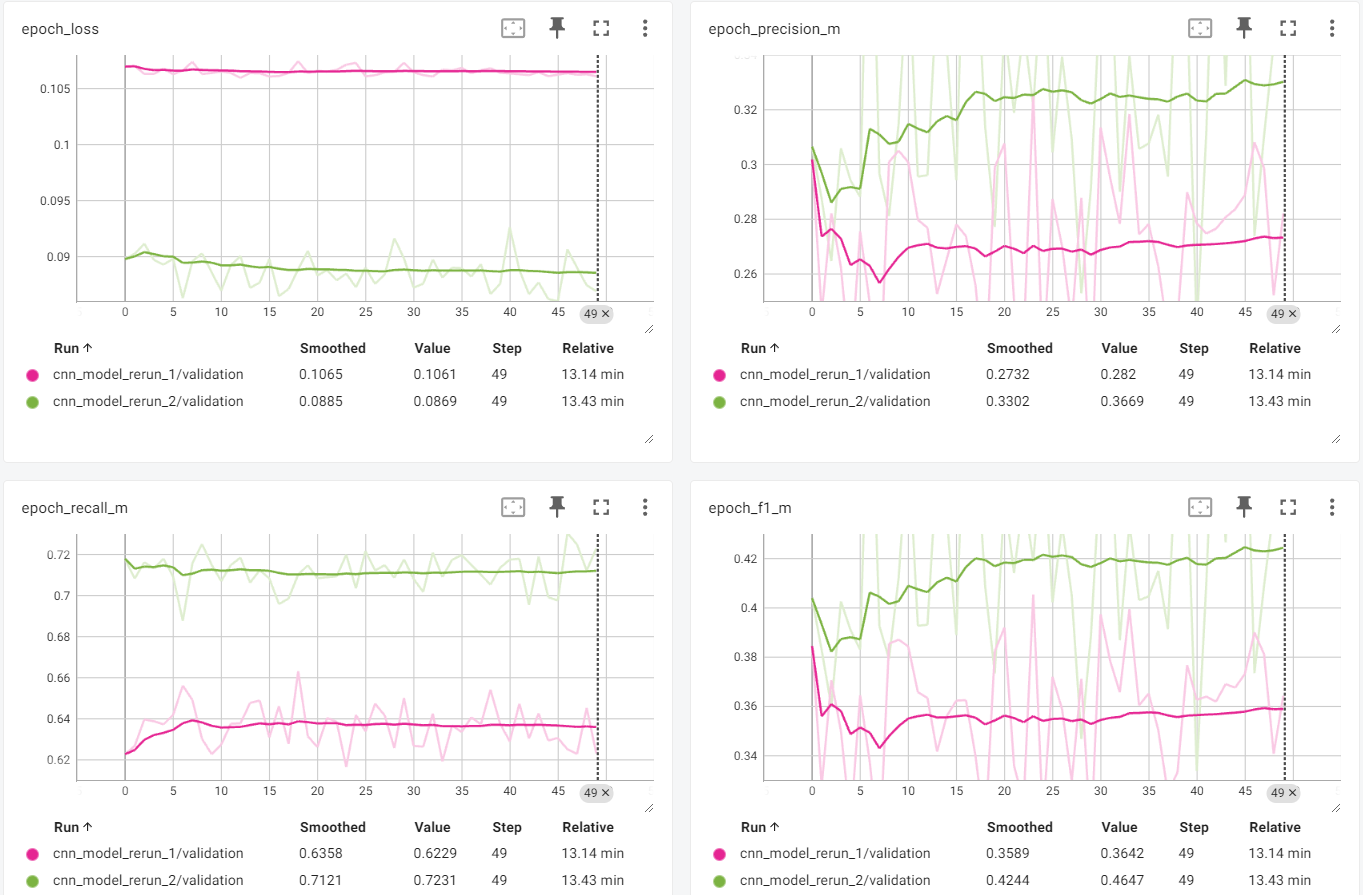
\includegraphics[width=1.2\linewidth,center]{MetricsResults.png}
	\caption[Différence de métriques entre deux CNN]{Différence de métriques entre deux CNN (en rose le premier CNN à régression et en vert le meilleur CNN testé).}
\end{figure}

Le meilleur \gls{cnn} trouvé travaille sur une fenêtre de 21 échantillons au lieu de 7, contient une couche de BatchNormalisation,
effectue des convolutions sur 11 échantillons au lieu de 4 et a une couche dense de 32 neurones au lieu de 16.

Cependant, on peut constater que même ce \gls{cnn} peine à performer avec une précision de seulement $~30\%$ et un Recall de $~70\%$.


\subsection{Entraînement avec Sample Weights}
Lors des tests avec différentes architectures de \gls{cnn}, un problème plus subtil a été trouvé.
Lors de l'entraînement d'un réseau, il est nécessaire d'avoir un dataset d'entraînement uniforme sur les différents cas qu'il verra lors de son utilisation.
Par exemple, si un réseau classifiant des habits n'est entraîné qu'avec un dataset contenant des chaussures à $99\%$ et que le $1\%$ 
restant se rapporte à d'autres types d'habits, celui-ci aura alors du mal à apprendre de ce $1\%$.

Dans des cas moins graves qu'une répartition 99/1, comme par exemple : une répartition 60/40, ce genre de disparités
des données peut être mitigé en utilisant des poids pour chaque cycle d'apprentissage. Les données apparaissant le plus souvent 
se verront attribuer un poids "léger" lors de l'apprentissage, car chaque rencontre avec une donnée appartenant 
aux $60\%$ est moins importante qu'une rencontre avec des données composant les $40\%$ restants, qui se voient attribuer un poids plus "lourd".

Dans notre cas, cela s'est représenté sous la forme des différentes valeurs des \gls{pe} détectés. 
Le nombre d'échantillons ne contenant aucun \gls{pe} était parfois en surnombre de plus de 3 fois comparé aux autres valeurs. 
J'ai alors créé une fonction calculant l'importance d'une fenêtre en fonction du nombre total de \gls{pe} qui y sont présents.

Malheureusement ces nouveaux poids ont eux l'effet inverse lors de l'entraînement des réseaux :
\begin{figure}[tbph!]
	\centering
	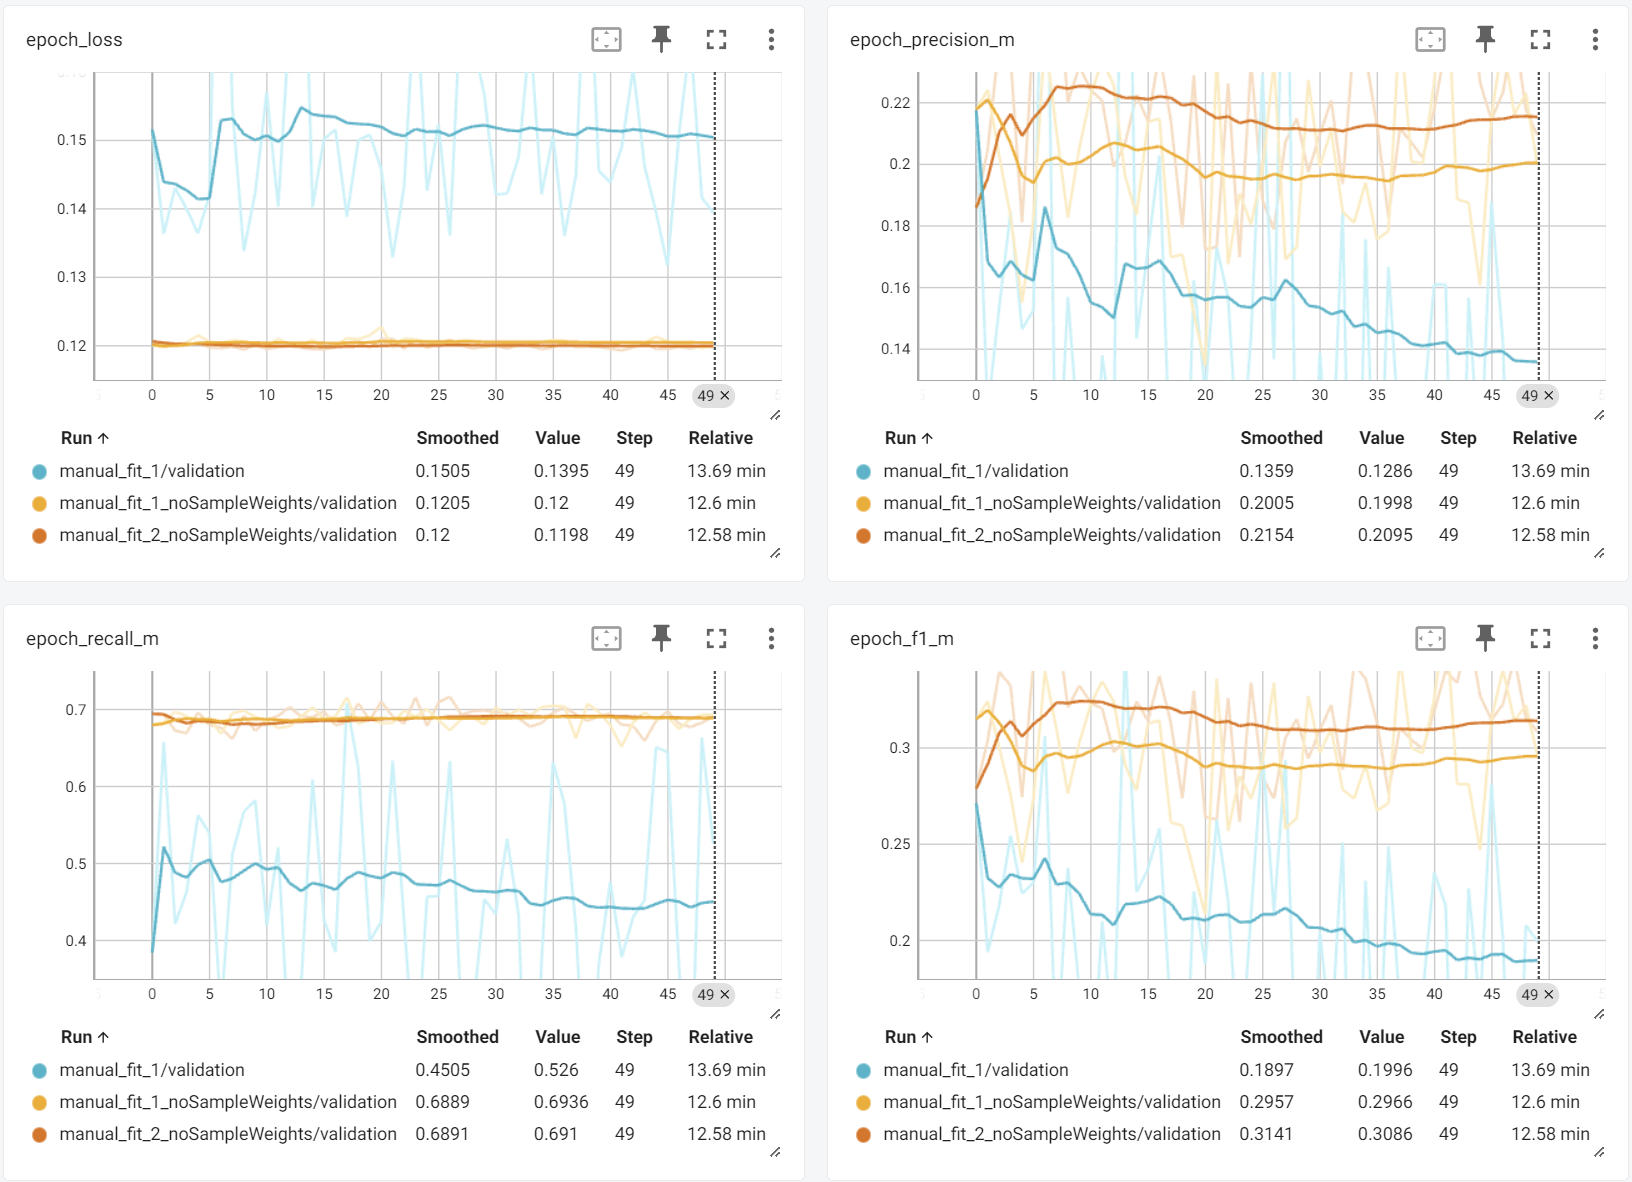
\includegraphics[width=1.1\linewidth,center]{SampleWeightsTraining.png}
	\caption[Perte de performance en entraînant avec des Sample Weights]{Perte de performance en entraînant avec des Sample Weights (en orange/jaune deux réseaux CNN entraînés sans Sample Weights, en bleu un modèle entraîné avec Sample Weights).}
\end{figure}

J'estime que cela est dû à l'application des Sample Weights sur une fenêtre complète. Une fenêtre peut contenir 
une grande proportion d'échantillons où aucun \gls{pe} n'est présent. Cela signifie que tous ces résultats sont 
quand même majorés par rapport au Sample Weight de la fenêtre et cela fausse donc l'apprentissage du réseau.

\subsection{Tests d'architecture RNN}
Pour essayer d'augmenter la précision ainsi que le Recall des derniers modèles testés, j'ai créé une architecture de \gls{rnn} simple ressemblant à ceci :

\begin{figure}[tbph!]
	\centering
	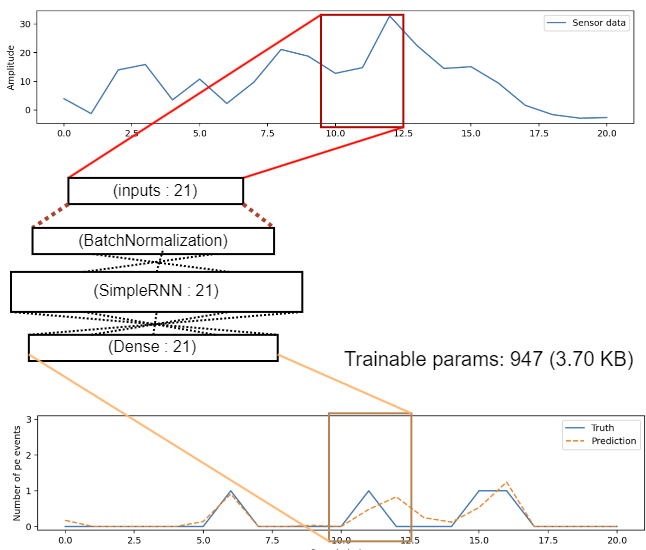
\includegraphics[width=0.8\linewidth]{RnnDiagram.drawio.png}
	\caption[Diagramme d'architecture du RNN simple]{Diagramme d'architecture du RNN simple.}
\end{figure}

Dès les premiers cycles d'entraînement, ce modèle \gls{rnn} s'est directement départagé des autres en achevant
très rapidement les meilleures performances sur les données simulées par "pe\_extractor" avec une précision de 
presque $~60\%$ et un Recall de $~70\%$ :
\newpage
\begin{figure}[tbph!]
	\centering
	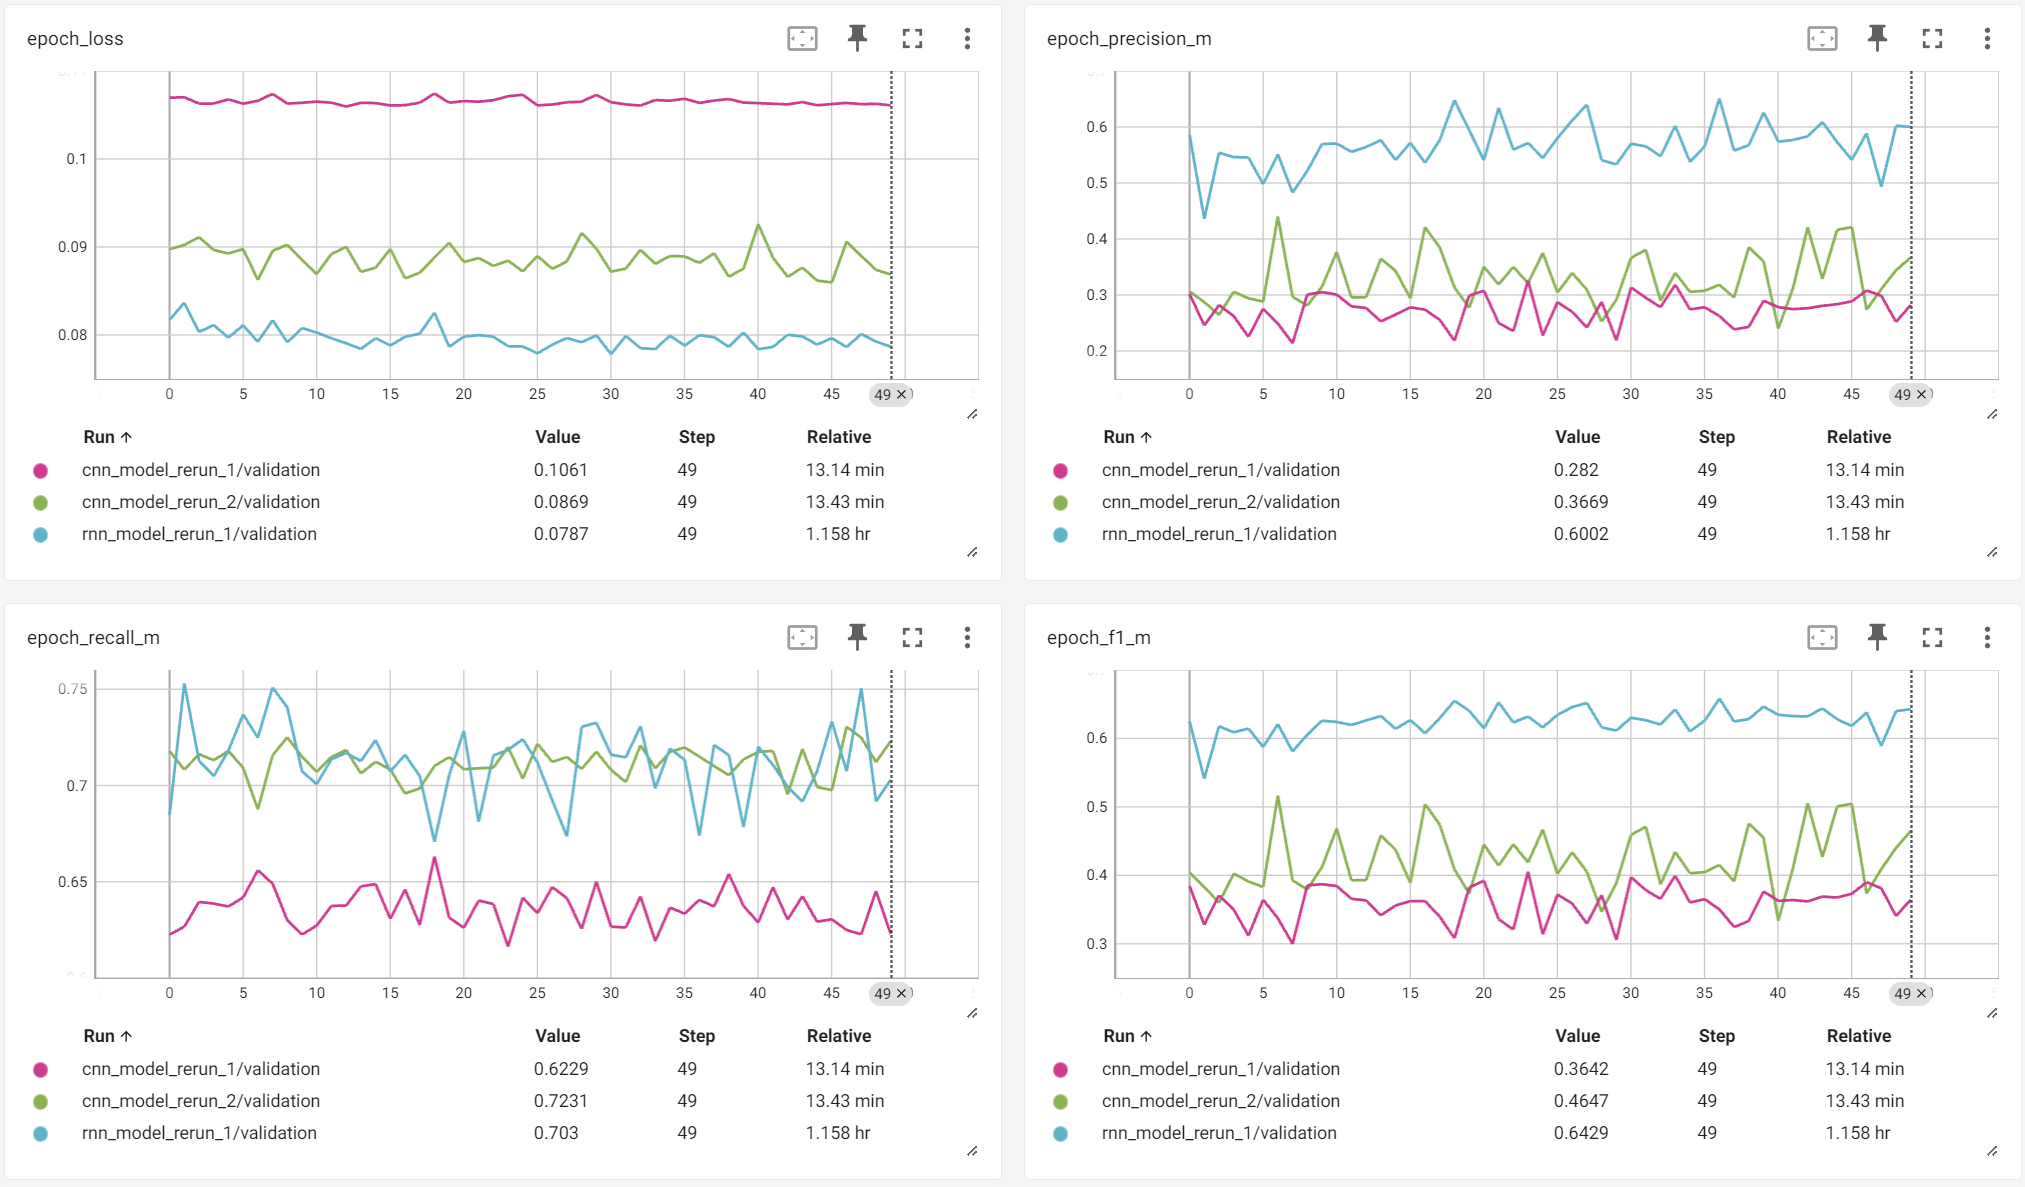
\includegraphics[width=1.2\linewidth,center]{RNNTraining.png}
	\caption[Comparaison des métriques entre CNN et RNN]{Comparaison des métriques entre CNN et RNN (en rose et vert les CNN et en bleu le RNN simple).}
\end{figure}

\section{Fichiers de simulation Corsika}
Après avoir testé de nombreuses autres configurations sur les données du précédent simulateur, j'ai pensé que 
les différents plateaux atteints lors des entraînements pouvaient être causés par les données elles-même.

J'ai pensé qu'en utilisant des données provenant de simulations plus complexes et 
avec des vraies pluies Cherenkov, cela pourrait aider les réseaux à y trouver des 
motifs qui n'existaient pas dans l'ancienne simulation.

L'équipe de l'\gls{unige} m'a alors fourni des fichiers de simulations pour la prochaine caméra du \gls{lst}.
Pour pouvoir utiliser ces fichiers, il a d'abord fallu recréer les signaux avec l'outil complémentaire : "pyeventio\_example".
Sur le cluster Yggdrasil, j'ai compilé et utilisé l'exécutable "runana" de manière distribuée grâce à un script bash :

\begin{lstlisting}[language=iBash,caption={Script de génération des signaux à partir de fichier de simulations, data/slurm-run.sh},captionpos=b]
#!/bin/sh

# manage cluster modules
module purge
module load GCC/11.2.0  OpenMPI/4.1.1 ROOT/6.24.06

# select events range to generate
ev_start=0
ev_stop=1000

# select the simulation file
inRootFiles="/srv/beegfs/scratch/shares/heller/Leonid/mono-lst-sipm-pmma-3ns-v1_triggerless/gamma/0000/corsika_0000ID.root"
rndseed="1312312"

for ((evID=ev_start; evID<=ev_stop; evID++))
do
	# location of output file
	binFileOut="/home/users/p/perrinya/scratch/bin_data/gamma_ev"$evID"_out.bin"
	# recreate complete waveform with truths
	srun --time "00:00:30" /home/users/p/perrinya/pyeventio_example/runana 333 "$inRootFiles" "$evID" "$binFileOut" "$rndseed" &
done
\end{lstlisting}

Les fichiers binaires créés utilisent bien plus de place que les fichiers ROOT. Par exemple, le fichier "corsika\_0000ID.root", comportant les
informations nécessaires à reconstruire environ $500'000$ pluies Cherenkov d'une durée d'environ $75ns$ chacune, ne pèse que $1.2GB$.
En comparaison, les $1'000$ premières pluies sous forme de fichiers binaires prennent plus de $2.38GB$ de stockage. 
Si l'on venait a stocker la totalité des événements d'un seul fichier ROOT en fichiers binaires,
ceux-ci prendraient une taille de : $500'000/1000 * 2.38GB = 1.19TB$

\newpage
Cependant, la création de ces fichiers n'est que la première étape pour créer un jeu de données utilisable par nos réseaux de neurones.
Les fichiers produits sont structurés de la manière suivante :
\begin{figure}[tbph!]
	\centering
	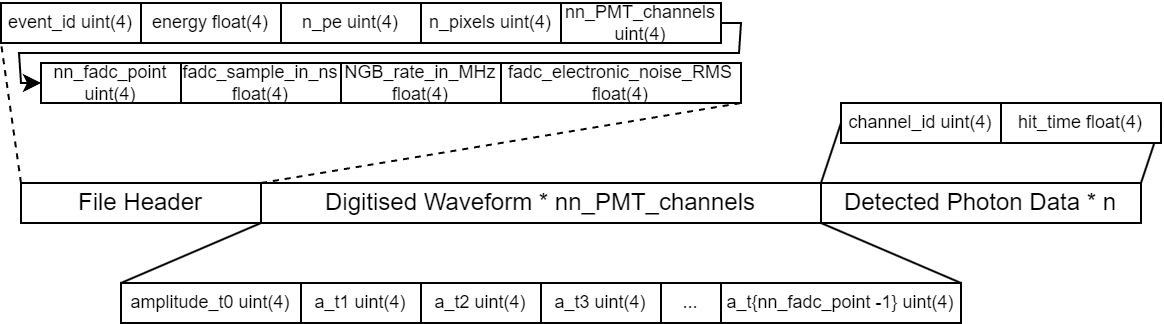
\includegraphics[width=\linewidth]{Pyeventio_binary_file_content.drawio.png}
	\caption[Structure des fichiers binaires de simulations Corsika]{Structure des fichiers binaires de simulations Corsika.}
\end{figure}

J'ai donc dû créer un lecteur capable de parser ces fichiers binaires et de recréer une vérité sur la même fréquence que le signal d'entrée.
Pour cela, la lecture du header et du signal se fait simplement en lisant et stockant des variables dans des tableaux en mémoire.
Cependant, quelques calculs et vérifications doivent être effectués pour les photons détectés par la caméra. 
En premier, il faut convertir l'instant de l'impact en numéro d'échantillon en divisant ce temps par la période d'acquisition connue dans l'entête du fichier.
Puis, il faut vérifier si ce photon a bien été capturé pendant la durée du signal, car celui-ci peut avoir été détecté
avant ou après l'événement, son temps d'impact peut donc être négatif ou supérieur à $75ns$, qui correspond la fin de la capture du signal.

\newpage
Au final, les données récupérées dans ces fichiers binaires sont similaires au premier simulateur :
\begin{figure}[tbph!]
	\centering
	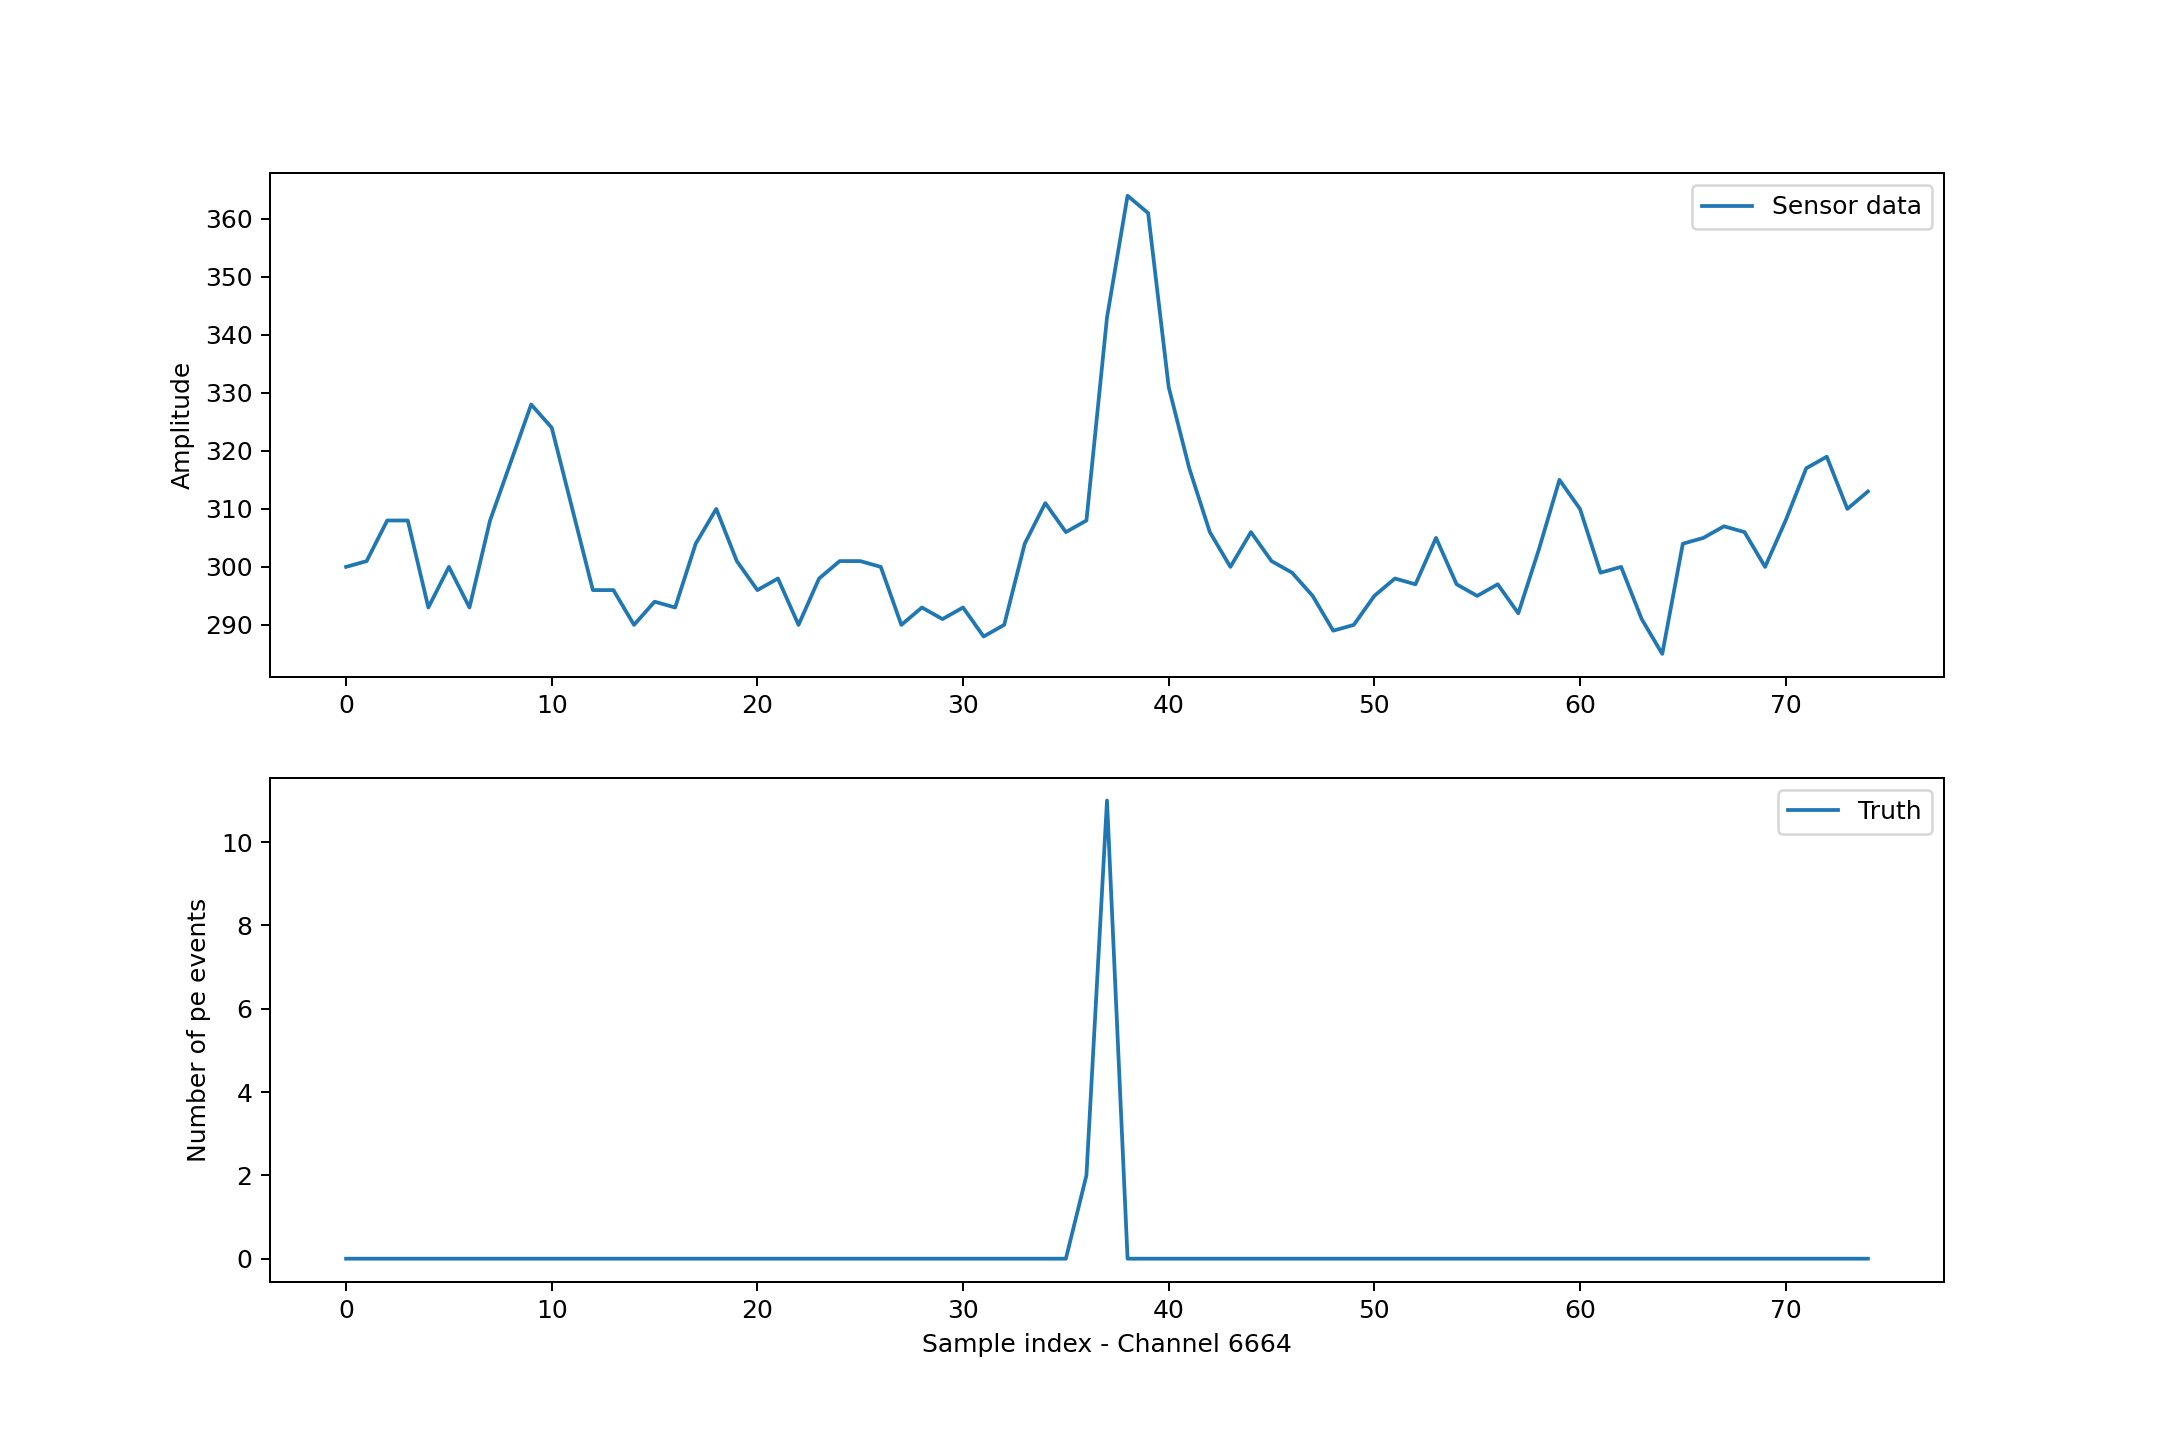
\includegraphics[width=\linewidth]{BinaryRecomposedSignalTruth.png}
	\caption[Exemple de données générées par simulations Corsika]{Exemple de données générées par simulations Corsika.}
\end{figure}

Cependant, même dans cet état, les données ne sont pas encore utilisables. Lorsque l'on regarde l'amplitude 
du signal contenu dans ces fichiers binaires, ceux-ci sont encodés sur des entiers. Pour réduire ces valeurs avant d'essayer
d'entraîner des réseaux neuronaux, il m'a été conseillé de normaliser ces données en les divisant par 8,5 en rapport avec les
capteurs simulés.

De plus, nous avons découvert que les temps d'impacts des photons détectés étaient un peu en avance par rapport
au signal. Nous avons donc ajouté un délai de 2 échantillons lors du parsing du fichier, pour que les pics de vérité arrivent en 
même temps ou avec un léger retard pour que le réseau de neurones puisse utiliser les échantillons précédents comme information utile.
\newpage
\begin{figure}[tbph!]
	\centering
	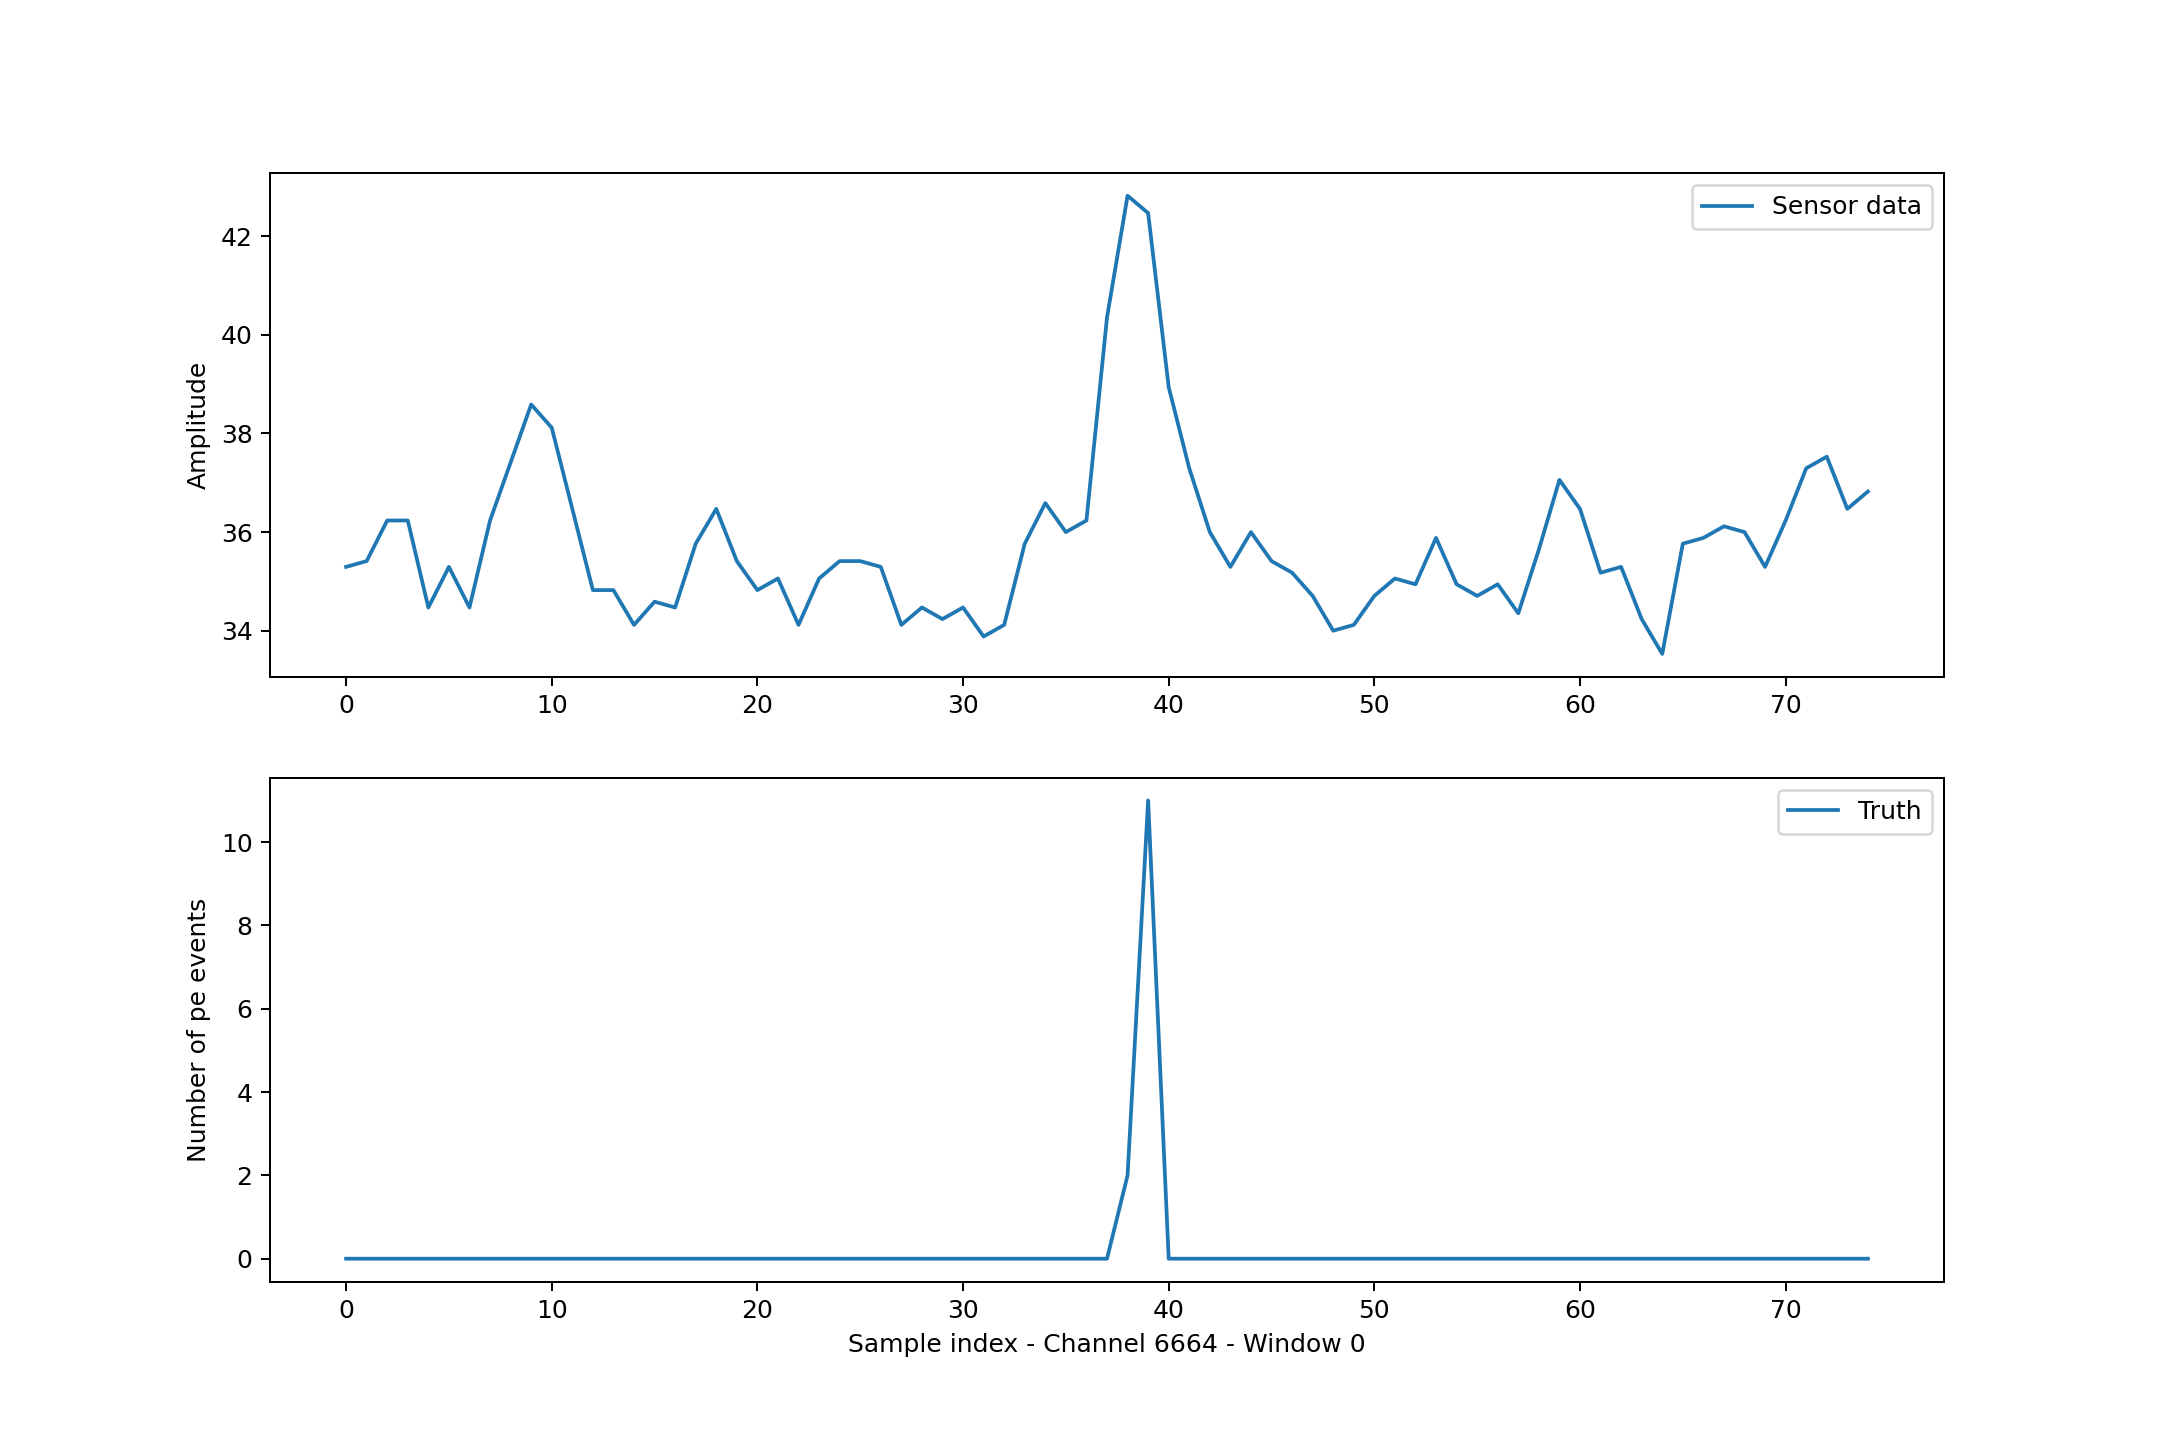
\includegraphics[width=\linewidth]{BinaryRecomposedSignalTruthNormalized.png}
	\caption[Données Corsika normalisées]{Données Corsika normalisées.}
\end{figure}

\newpage
\subsection{Création d'un dataset}
Ici aussi, comme pour le simulateur "pe\_extractor", il a été nécessaire de créer un dataset à partir des données brutes.
Cependant, pour ces fichiers de simulations, les signaux reconstitués à partir des fichiers binaires ne forment pas un seul long
signal mais $7'855$ signaux de $~75ns$ chacun. Il est donc nécessaire de prendre chaque signal à part individuellement 
pour créer des fenêtres capables d'entraîner les réseaux de neurones.

Lors de la création de ce nouveau dataset, un problème d'uniformité encore plus grave que le simulateur "pe\_extractor" a été constatée.
Les pluies Cherenkov sont des événements très brefs et peu énergétiques. Cela est d'autant plus vrai pour le \gls{lst} 
qui est le télescope le plus sensible de la nouvelle génération.

Tous les signaux concaténés d'une pluie Cherenkov ressemblent à ceci :
\begin{figure}[tbph!]
	\centering
	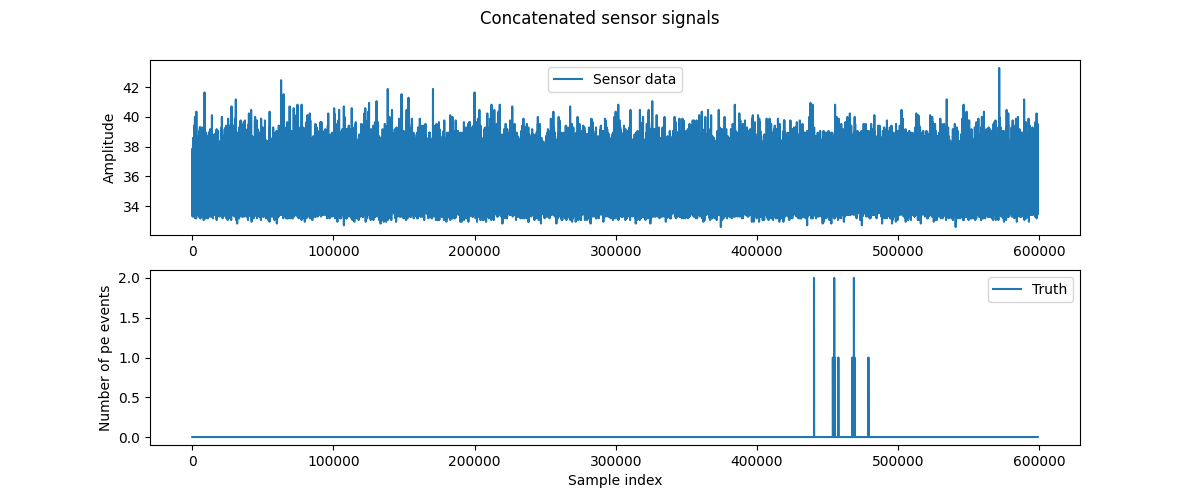
\includegraphics[width=\linewidth]{CorsikaSparsePe.png}
	\caption[Signaux concaténés de chaque capteur d'une pluie Cherenkov]{Signaux concaténés de chaque capteur d'une pluie Cherenkov.}
\end{figure}

\newpage
Pour éviter ce problème, alors que les Sample Weights n'avaient pas l'air de donner de bons résultats précédemment,
j'ai ajouté, lors de la création d'un dataset, une limite sur le nombre de fenêtres contenant un même nombre de \gls{pe}. 
Afin d'éviter que ce ne soit toujours les $x$ premières fenêtres d'un événement qui soient sélectionnées, chaque fenêtre est choisie de manière aléatoire.
Avec cette limitation, le dataset généré est beaucoup plus uniforme :
\begin{figure}[tbph!]
	\centering
	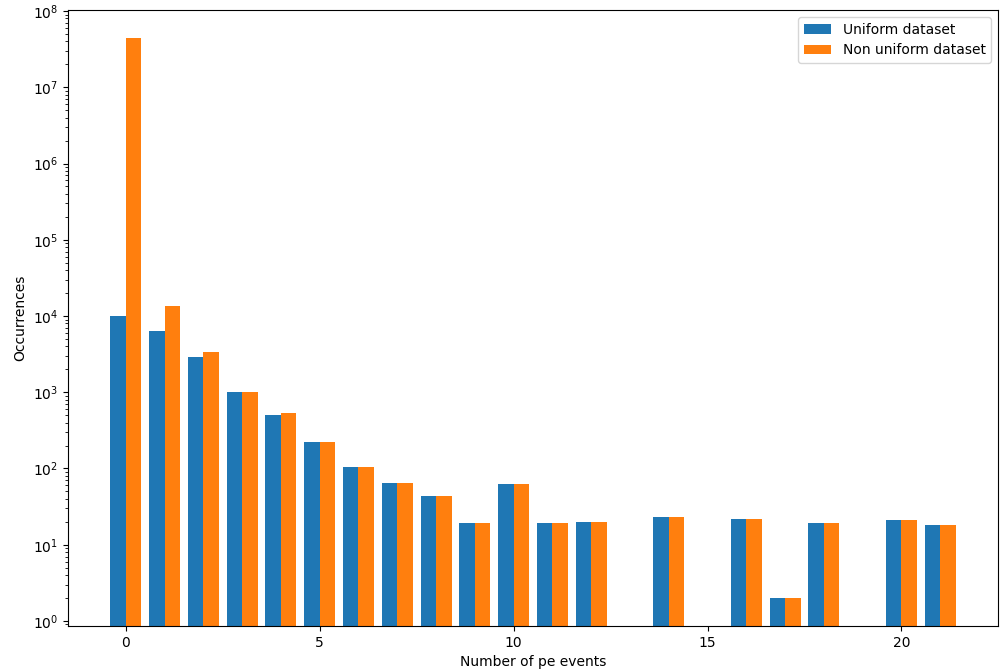
\includegraphics[width=0.8\linewidth]{UniformDatasetDistributionComparaisonCrop.png}
	\caption[Comparaison entre un dataset uniformisé et non uniformisé générés sur 100 pluies Cherenkov]{Comparaison entre un dataset uniformisé et non uniformisé générés sur 100 pluies Cherenkov.}
\end{figure}

Cela réduit la taille du dataset considérablement, ce qui permet de le stocker et de le garder en mémoire vive plus facilement.
Le dataset créé pour les entraînements contient lui les $1'000$ premières pluies simulées du fichier Corsika :
\begin{figure}[tbph!]
	\centering
	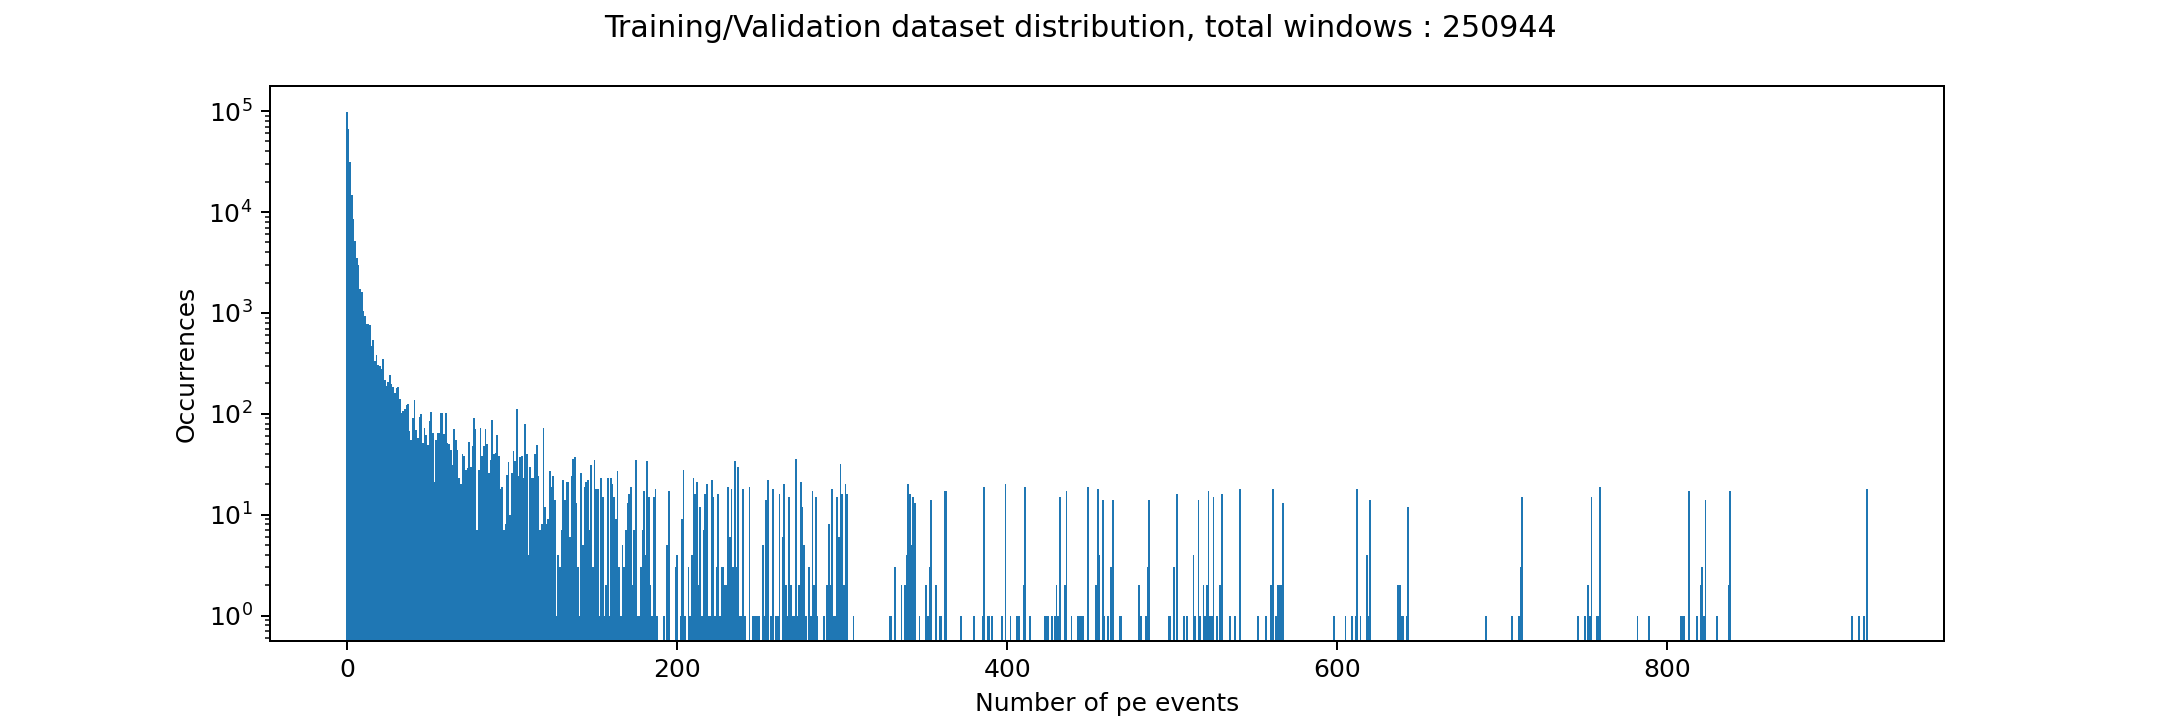
\includegraphics[width=\linewidth]{CorikaTrainingDatsetDistribution.png}
	\caption[Distribution du dataset généré pour les entraînements]{Distribution du dataset généré pour les entraînements.}
\end{figure}

Pour éviter de devoir à chaque fois recharger et traiter ces $1'000$ événements, j'ai aussi créé un système de sauvegarde et chargement d'un dataset.

\subsection{Entraînement des réseaux de neurones}
Avec ce nouveau dataset, j'ai repris les différentes architectures de réseaux qui avaient donné les meilleurs résultats sur l'ancien simulateur.
J'ai ensuite relancé des entraînements de zéro et ai observé les résultats suivants :

\begin{figure}[tbph!]
	\centering
	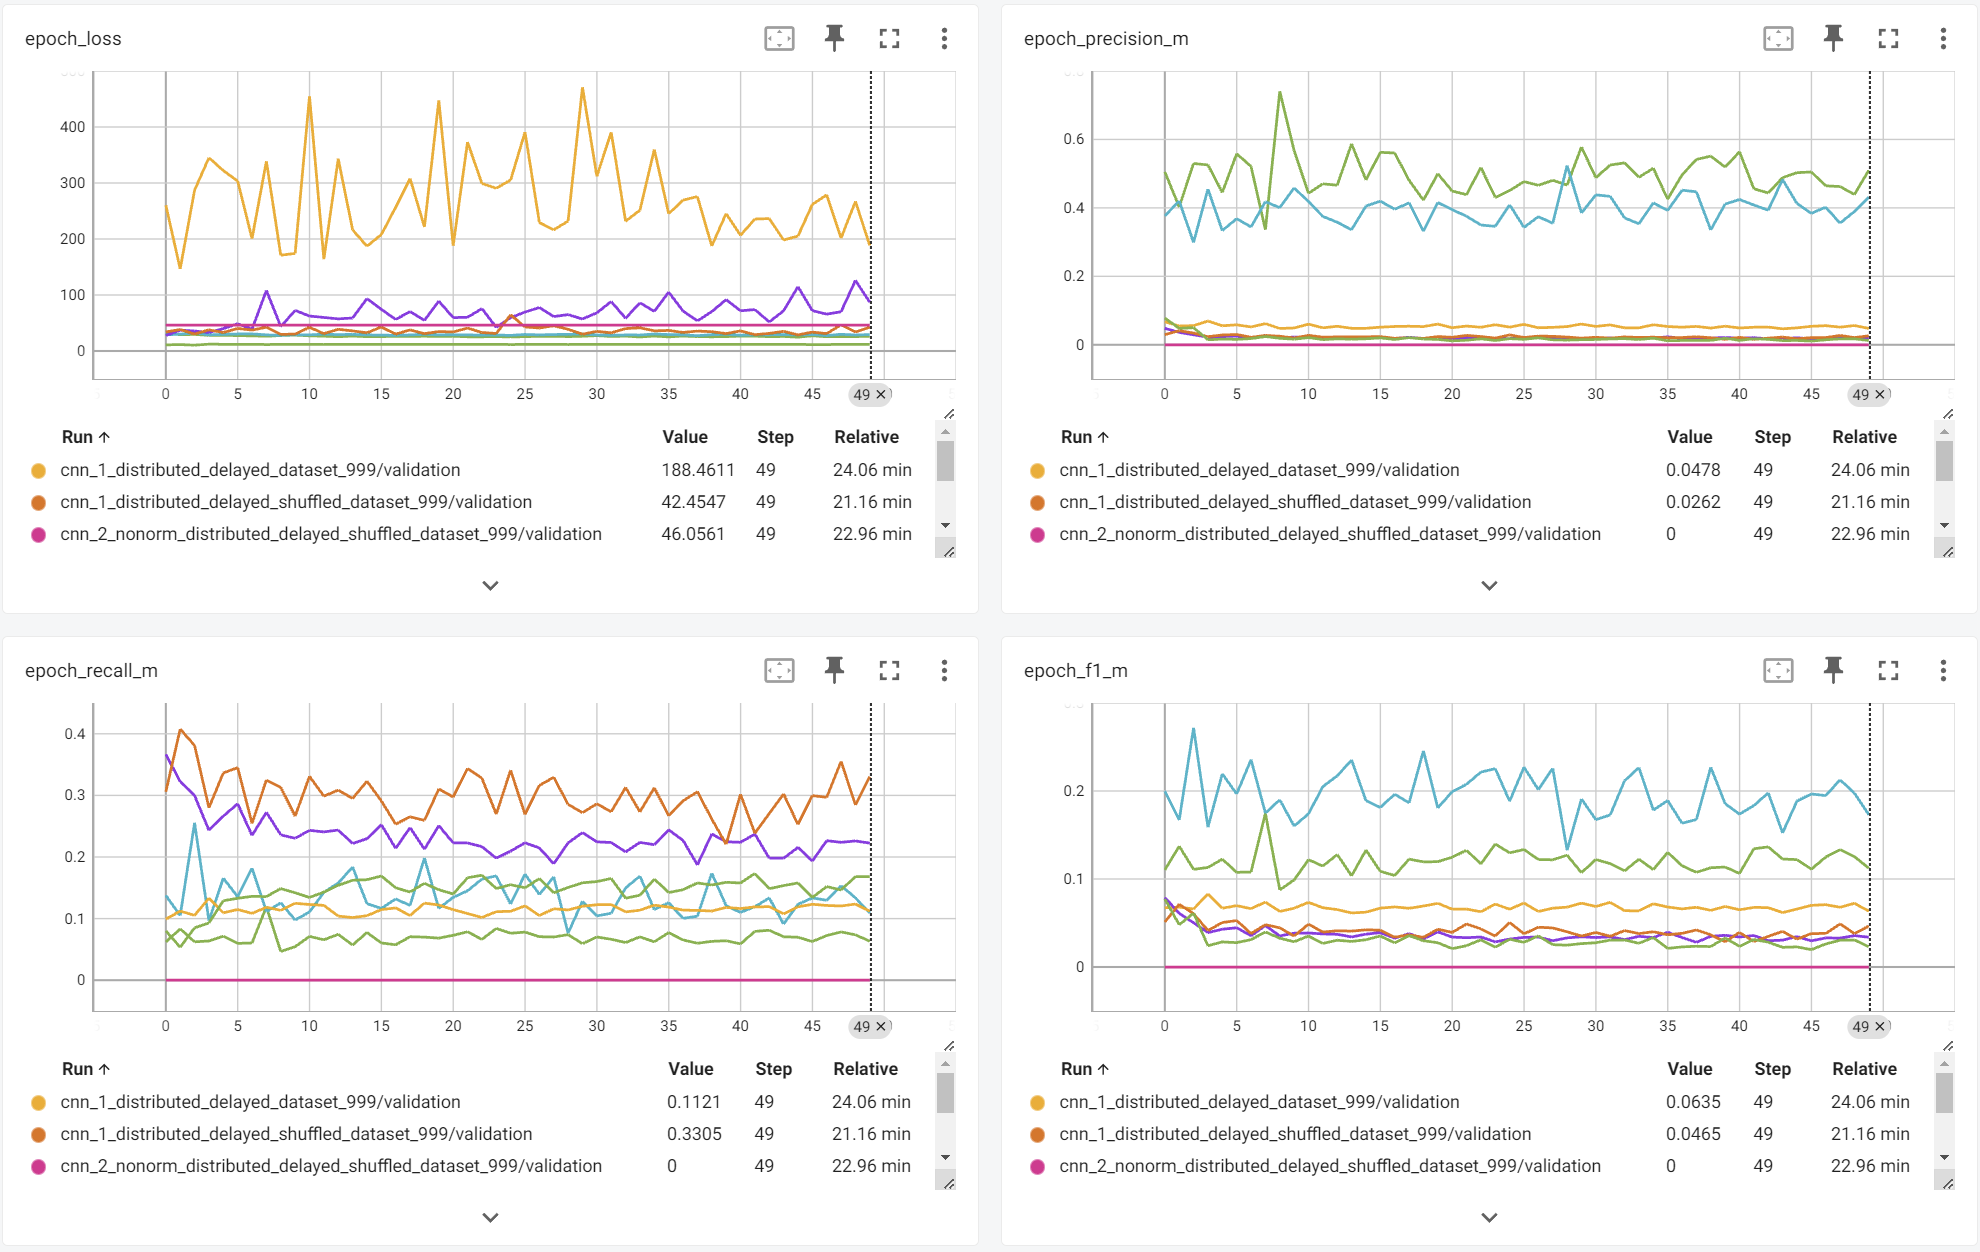
\includegraphics[width=1.2\linewidth,center]{CorsikaTraining.png}
	\caption[Métriques d'entraînement des modèles sur les données Corsika]{Métriques d'entraînement des modèles sur les données Corsika.}
\end{figure}

Les résultats de ces entraînements ont régressés par rapport au simulateur "pe\_extractor". 
Après analyse, je pense que cela est dû aux données du simulateur et aux différentes limitations physiques des capteurs.
Lorsque l'on regarde de près certaines fenêtres du dataset, on constate que les petites quantités de \gls{pe} présentes dans le signal
ne participent que très peux à l'amplitude de celui-ci, rendant l'extraction de l'information difficile.
\newpage
\begin{figure}[tbph!]
	\centering
	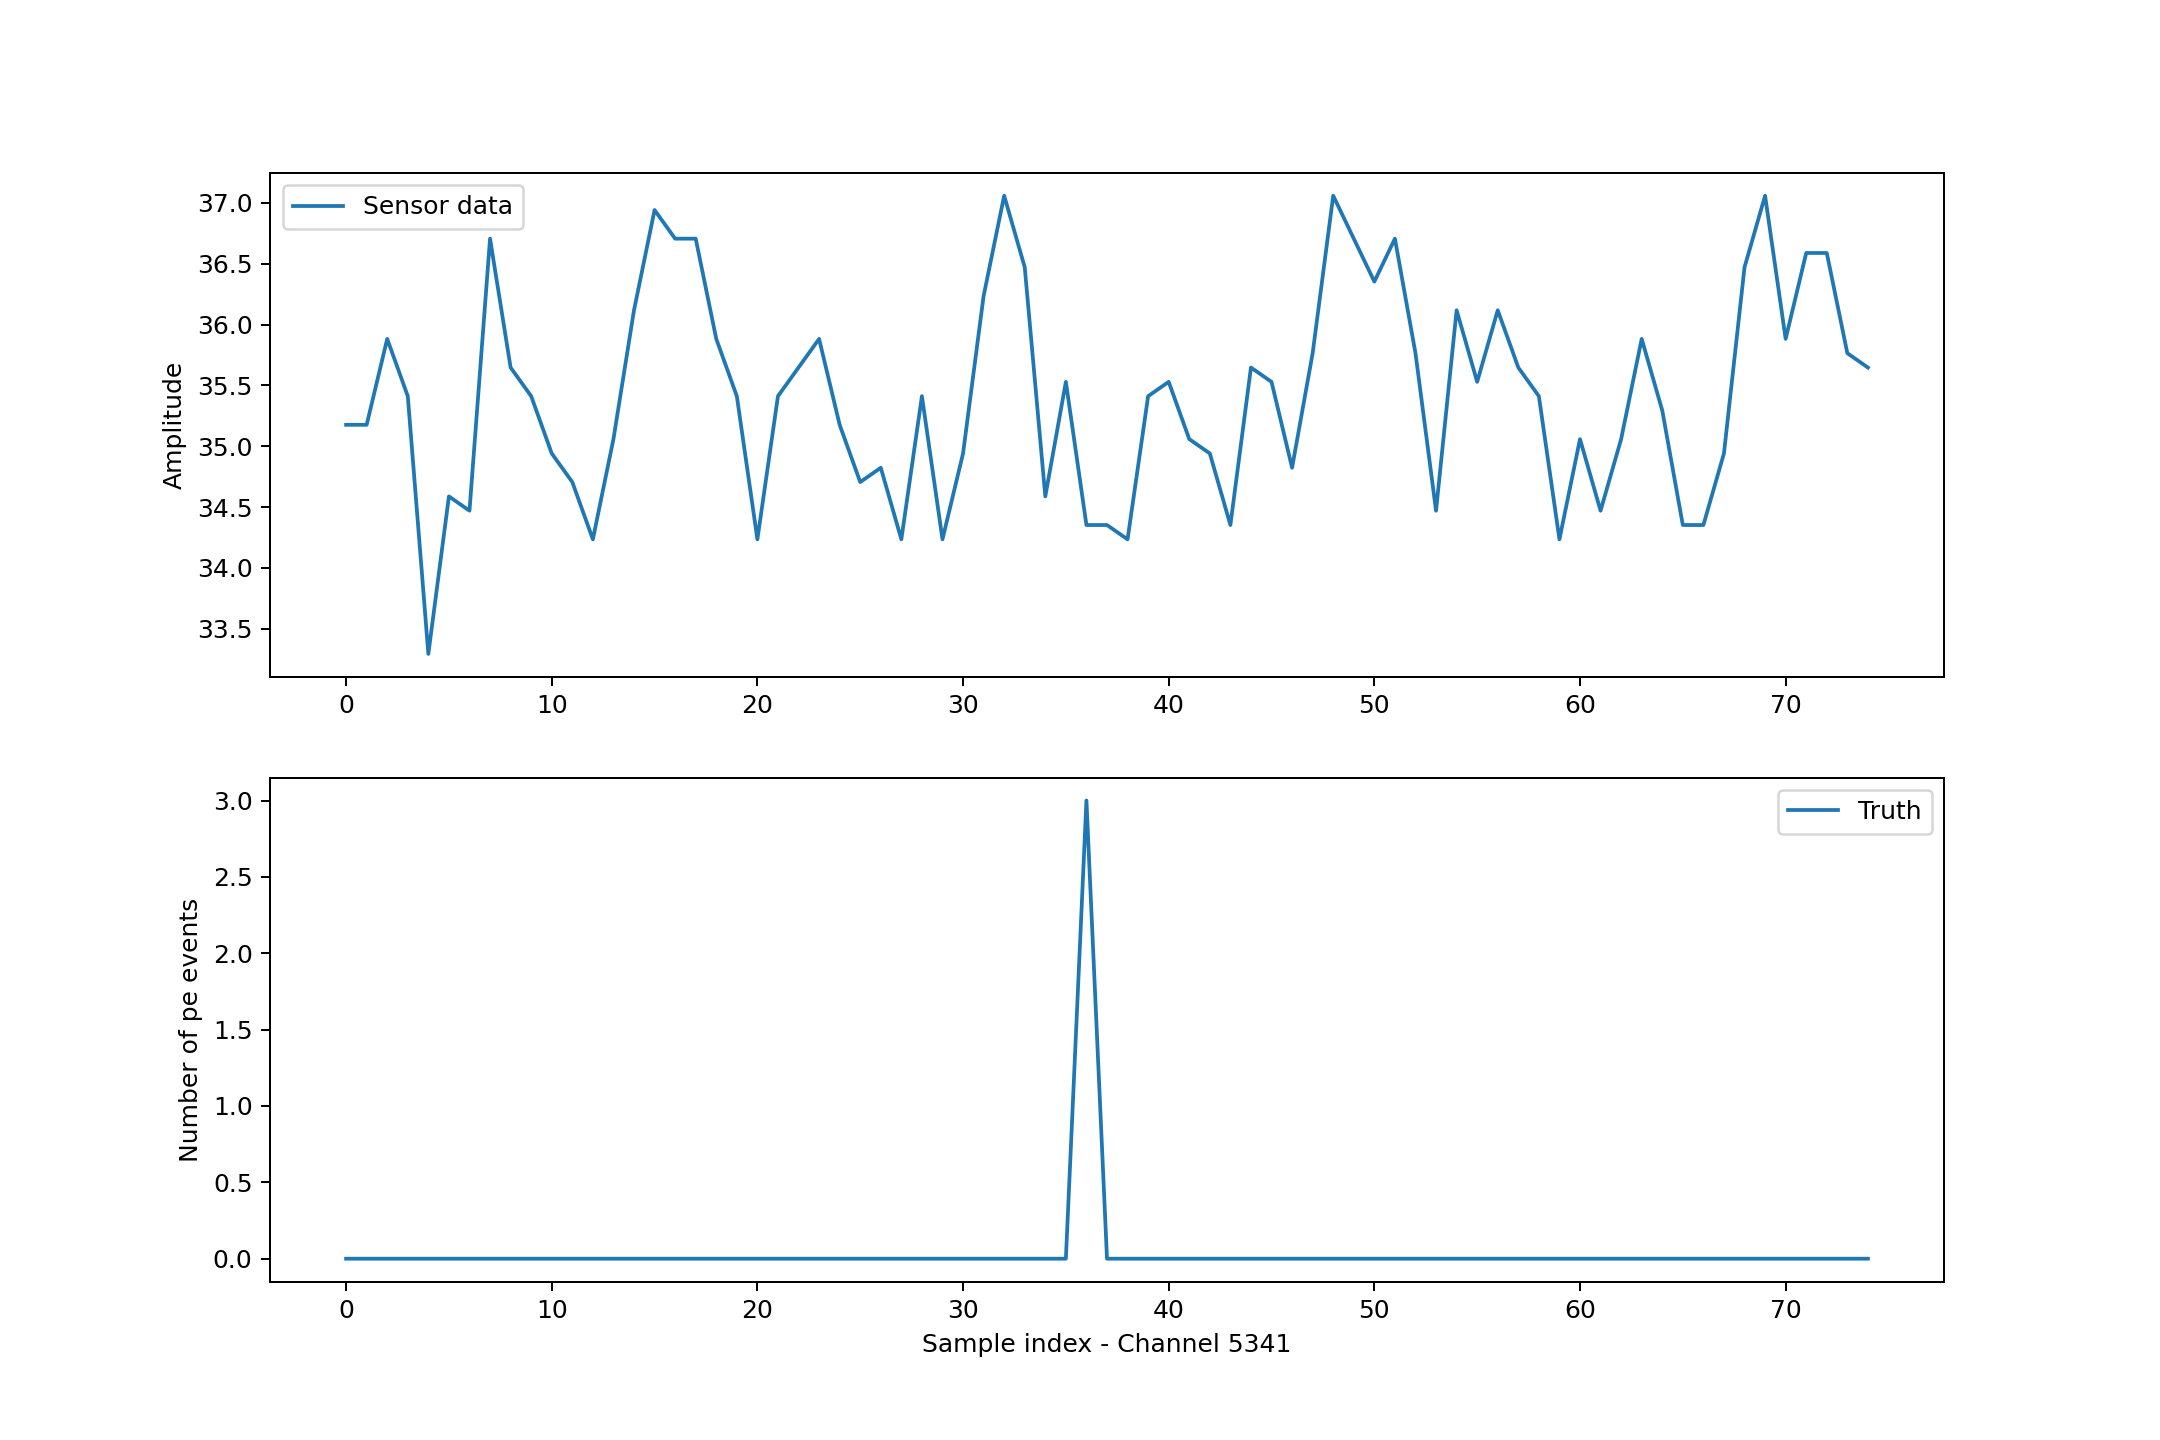
\includegraphics[width=\linewidth]{CorsikaDataProblemsExample.png}
	\caption[Exemple de données Corsika difficilement discernables]{Exemple de données Corsika difficilement discernables.}
\end{figure}

Ici, le pic d'amplitude produit par la présence des 3 \gls{pe} présents dans le signal est difficilement discernable du bruit alentour.
La forme du pic pourrait être discernable par un réseau de neurones mais la faible résolution temporelle 
disponible dans ces échantillons me fait douter de la possibilité d'en tirer des informations concluantes sur 
des petites quantités de \gls{pe}.

\section{Améliorations possibles}
C'est malheureusement à ce point que je n'ai pas réussi à explorer de techniques supplémentaires pour pallier aux problèmes 
rencontrés lors de l'utilisation de données plus proches des capteurs réels. Cependant, il me reste encore une idée qui 
pourrait possiblement réduire les problématiques rencontrées.

Lors de pluies atmosphériques Cherenkov, plusieurs capteurs aux alentours sont souvent aussi touchés.
Le bruit électronique de chaque capteur est majoritairement propre à lui même. Même si une partie de 
l'électronique produit du "CrossTalk" qui est du bruit électrique se propageant autour de chaque pièce matérielle, 
celui-ci pourrait être amoindri en analysant non plus un pixel seul mais un groupe de pixels voisins.